%%%%%%%%%%%%%%%%%%%%%%%%%%%%%%%%%%%%%%%%%%%%%%%%%%%%%%%%%%%%%%
%% 卒論サンプル 2015.10.26, ... 2024.12.13 改 I. (template author)
%%・ラベルを使っているので TeX に2回かけること！
%% （T2P または T2R ボタン）
%%・「titlepage_a4j.tex」と「卒業論文閲覧承諾書.pdf」ファイルを同じフォルダに置いておくこと！
%%%%%%%%%%%%%%%%%%%%%%%%%%%%%%%%%%%%%%%%%%%%%%%%%%%%%%%%%%%%%%
\documentclass[a4j,12pt]{jarticle}
\usepackage{amsmath}          % AmS-LaTeX を使うなら
\usepackage{cases}        % numcases 環境のため
\usepackage{amsthm}         % 定理環境のため
\usepackage{bm}           % もしエラーになるならこの行は削除してもよい.
\usepackage{amssymb}          % AmS-LaTeX を使うなら
%\usepackage{type1cm}         % タイトルに数式を使うならここを有効にして！

\usepackage[dvipdfmx]{graphicx}
\usepackage{booktabs}         % \toprule, \midrule, \bottomrule を使うために必要
\usepackage{float}

%% 定理環境の定義
% テキストp.46「§2.4.2 定理環境の定義」参照
\theoremstyle{definition}
\newtheorem{theorem}{定理}[section]
%\newtheorem{theorem}{定理}   % セクション番号を付けないならこちら
\newtheorem*{theorem*}{定理}  % * 付きは定理番号が付かない
\newtheorem{lemma}[theorem]{補題}
\newtheorem{corollary}[theorem]{系}
\newtheorem{definition}[theorem]{定義}
\newtheorem{example}[theorem]{例}

\newtheorem{proof_sketch}{証明の概略}

%% 証明環境
\renewcommand{\proofname}{(証明)}
\renewcommand{\topfraction}{1.0}    % ページ上部の図の割合（最大100%）
\renewcommand{\bottomfraction}{1.0} % ページ下部の図の割合（最大100%）
\renewcommand{\textfraction}{0.0}   % 最小限必要な本文の割合（0%でもOK）
\renewcommand{\floatpagefraction}{1.0} % 図専用ページの最小割合
% 必要ならば{(証明)}を{\textbf{証明.}}等と変更することもできる.
\makeatletter
\renewenvironment{proof}[1][\proofname]{\par
  \pushQED{\qed}
  \normalfont \topsep6\p@\@plus6\p@\relax
  \trivlist
  \item[\hskip\labelsep #1]\ignorespaces
}{
  \popQED\endtrivlist\@endpefalse % 証明終了の記号□を最後に付ける
% \endtrivlist\@endpefalse        % □を付けないようにしたければこちら
}
\makeatother
% 数式の番号をセクション番号なしにしたければ, 次の式をコメントアウト(削除)する.
% （amsmath を仮定している）
\numberwithin{equation}{section}

%% 関数記号の定義例（amsmath を仮定している）
%% 添え字を使う命令には * を付ける：
\DeclareMathOperator{\End}{End}
\DeclareMathOperator{\Ker}{Ker}

%% 数式中の太字とブラックボードボールド体の定義
% 数式中の太字は $ \bm{v} $ などとすればよい.
% 複素数体は $ \CC $, 整数全体は $ \ZZ $ とかける.
\providecommand{\bm}[1]{\boldsymbol{#1}}
\providecommand{\bmdefine}[2]{\newcommand{#1}{\bm{#2}}}
\newcommand{\CC}{\mathbb{C}}
\newcommand{\RR}{\mathbb{R}}
\newcommand{\QQ}{\mathbb{Q}}
\newcommand{\ZZ}{\mathbb{Z}}
% よく使う太字はプリアンブル(この近所)に
% \bmdefine{\bv}{v}
% 等と定義しておいて, 本文中は $ \bv $ 等とすることもできる.

%%%%%%%%%%%%%%%%%%%%%%%%%%%%%%%%%%%%%%%%%%%%%%%%%%%%%%%%%%%%%%
%% サンプルの卒業年度, 論文題目, 指導教員名を消して
%% 自分の卒業年度, 論文題目, 氏名, 指導教員名をかくこと.
%%%%%%%%%%%%%%%%%%%%%%%%%%%%%%%%%%%%%%%%%%%%%%%%%%%%%%%%%%%%%%
\newcommand{\卒業年度}{7}
\newcommand{\論文題目}{最良近似多項式の導出と\\アルゴリズム}    %卒論テーマ
\newcommand{\氏名}{imohiyoko}        %名前
\newcommand{\指導教員}{（指導教員）}    %指導教員名
%%%%%%%%%%%%%%%%%%%%%%%%%%%%%%%%%%%%%%%%%%%%%%%%%%%%%%%%%%%%%%

\title{\論文題目}
\author{\氏名}
\date{} % 日付を表示しない場合は空にする

\begin{document}

\newpage  %% 改ページ ==================================================
%%%%%%%%%%%%%%%%%%%%%%%%%%%%%%%%%%%%%%%%%%%%%%%%%%%%%%%%%%%%%%
%% （大学名非公開）理学部数理科学卒業論文表紙(a4j用)
%% Ver. 0.92 (2015.10.26, I.K.) 
%% 2018.10.31改 (年号が平成から変わるかもしれないので移動した)
%%%%%%%%%%%%%%%%%%%%%%%%%%%%%%%%%%%%%%%%%%%%%%%%%%%%%%%%%%%%%%
%% 書き換えないこと！
%%%%%%%%%%%%%%%%%%%%%%%%%%%%%%%%%%%%%%%%%%%%%%%%%%%%%%%%%%%%%%
\thispagestyle{empty}
\begin{picture}(0,0)(140,705)

\put(202,656){
 \parbox[t]{300pt}{
  \fontsize{26pt}{20pt}\selectfont
  卒　　\,業　　\,論　　\,文
 }
}

\put(124,579){
 \parbox[t]{15cm}{%
  \fontsize{36pt}{50pt}\selectfont
  \begin{center}
   \論文題目
  \end{center}
 }
}

\put(200,190){
 \parbox[t]{300pt}{
  \kanjiskip=1pt
  \fontsize{20pt}{20pt}\selectfont
  \begin{tabular*}{.5\textwidth}{@{}l@{}l@{\ \,}l}
  卒業年度&：& \卒業年度\,\,年度\\[5mm]
  氏　　名&：& \氏名\\[5mm]
  指導教員&：& \指導教員
  \end{tabular*}
 }
}

\put(223,80){
 \parbox[t]{300pt}{
  \kanjiskip=0.8pt
  \fontsize{18pt}{18pt}\selectfont
	（大学名非公開）
 }
}

\end{picture}
 % 表紙を出力する
%%%%%%%%%%%%%%%%%%%%%%%%%%%%%%%%%%%%%%%%%%%%%%%%%%%%%%%%%%%%%%
%% （大学名非公開）理学部数理科学卒業論文表紙(a4j用)
%% Ver. 0.92 (2015.10.26, I.K.) 
%% 2018.10.31改 (年号が平成から変わるかもしれないので移動した)
%%%%%%%%%%%%%%%%%%%%%%%%%%%%%%%%%%%%%%%%%%%%%%%%%%%%%%%%%%%%%%
%% 書き換えないこと！
%%%%%%%%%%%%%%%%%%%%%%%%%%%%%%%%%%%%%%%%%%%%%%%%%%%%%%%%%%%%%%
\thispagestyle{empty}
\begin{picture}(0,0)(140,705)

\put(202,656){
 \parbox[t]{300pt}{
  \fontsize{26pt}{20pt}\selectfont
  卒　　\,業　　\,論　　\,文
 }
}

\put(124,579){
 \parbox[t]{15cm}{%
  \fontsize{36pt}{50pt}\selectfont
  \begin{center}
   \論文題目
  \end{center}
 }
}

\put(200,190){
 \parbox[t]{300pt}{
  \kanjiskip=1pt
  \fontsize{20pt}{20pt}\selectfont
  \begin{tabular*}{.5\textwidth}{@{}l@{}l@{\ \,}l}
  卒業年度&：& \卒業年度\,\,年度\\[5mm]
  氏　　名&：& \氏名\\[5mm]
  指導教員&：& \指導教員
  \end{tabular*}
 }
}

\put(223,80){
 \parbox[t]{300pt}{
  \kanjiskip=0.8pt
  \fontsize{18pt}{18pt}\selectfont
	（大学名非公開）
 }
}

\end{picture}
 % 表紙を出力する

\pagenumbering{roman}   % ページ番号をローマ数字にする.

% =========================================================
% 前付 (概要・目次)
% =========================================================

% 概要 (Abstract)
% ページ番号がローマ数字の間に配置します
\section*{はじめに}
\label{sec:introduction}
  \subsection*{研究の背景と目的}
    コンピュータは四則演算を行うことを前提として設計されているため，多項式の計算は高速に行うことができる．
    しかし，多項式で直接あらわすことができない関数（例えば指数関数や三角関数など）というのは多々存在する．

    そのため，そういった関数を多項式で近似することで，計算機上での数値計算の実行速度を高速化できるなどのメリットが生まれる．
    さて，近似多項式の作成にはいくつか知られた手法が存在する．
    例えば，テイラー展開は，指定した点付近での精度は極めて高いが，その点から離れるにつれて誤差が増大する．そのため，定義域内においての最大誤差の抑制が求められる場合には不向きである
    その対策として事前に設定した標本点を通る多項式であるラグランジュ補間多項式は，閉区間 $\left[a,b\right]$ における$n$次多項式を一意に決定することができる．
    しかし，煩雑な標本点を用いた場合など標本点の取り方によって求める誤差関数の最大ノルムよりも大きな誤差が生じる場合がある．
    そのため，ここではラグランジュ補間多項式を用いた多項式近似において誤差関数の最大ノルムを最小化した最良近似多項式とそれを取得するために必要となる標本点の導出手法，それによってどのような近似を得ることができるかについて考える．

  \subsection*{本論文の構成}
    \begin{list}{}{
        \setlength{\leftmargin}{4.5em} % 本文のインデント幅（「第X章」の幅+α）
        \setlength{\labelwidth}{4.5em} % ラベル「第X章」の幅
        \setlength{\itemindent}{0pt}   % 1行目のインデント補正
        \setlength{\labelsep}{0.5em}   % ラベルと本文の間隔
        \setlength{\itemsep}{1em}      % 項目ごとの隙間（ここを調整して広げられます）
    }

    \item[\textbf{第1章}]
    「ラグランジュ補間多項式とその評価」では，関数近似の基礎となる多項式補間の理論について述べる．
    特にラグランジュ補間について解説し，等間隔な標本点を用いた場合に発生するルンゲ現象の問題点について，具体的な数値例を用いて示す．

    \item[\textbf{第2章}]
    「最良近似多項式の理論」では，本研究の核心である最良近似の数学的基礎について述べる．
    一様ノルムによる誤差の定義，最良近似多項式の存在と一意性，そしてRemesアルゴリズムの収束判定条件となるチェビシェフの交替定理について解説する．

    \item[\textbf{第3章}]
    「Remesアルゴリズムによる最良近似多項式の計算」では，最良近似多項式を数値的に導出する手法について述べる．
    特に，反復ごとに参照点を更新する「全点同時入れ替え法」の手順と，その2次収束性について理論的な背景を説明する．

    \item[\textbf{第4章}]
    「極値点探索の手法」では，Remesアルゴリズムの収束性能を左右する誤差関数の極値探索に焦点を当てる．
    微分を用いずに高速な収束を実現するBrent法のアルゴリズム構成と，その根拠について説明する．

    \item[\textbf{第5章}]
    「Brent法を用いたRemesアルゴリズムの実装と評価」では，提案手法の実装詳細と数値実験の結果について述べる．
    ルンゲ関数 $f(x) = 1/(1+25x^2)$ を対象とした近似実験を行い，グリッド極値点探索を用いた従来手法と比較して，提案手法が機械イプシロン程度の精度で交替定理を満たす解を導出できることを定量的に示す．

    \item[\textbf{第6章}]
    「考察」では，数値実験の結果に基づき，グリッド極値点探索法とBrent法の性能差が生じた要因について数理的な観点から議論する．
    特に，各極値における残留誤差の定量評価を通じ，Brent法の導入がRemesアルゴリズムの理論的な2次収束性を実現するために不可欠であることを明らかにする．

    \item[\textbf{第7章}]
    「結論」では，本研究で得られた知見を総括し，今後の課題と展望について述べる．
    \end{list}
  \subsection*{謝辞}
    本研究を進めるにあたり，多大なるご指導とご助言をいただきました指導教員の先生に深く感謝いたします．
    また，有益な助言をいただいた研究室の皆様，そして在学中支えてくれた家族に心より感謝申し上げます．
\newpage  %% 改ページ ==================================================

% 目次
\tableofcontents
\clearpage

% =========================================================
% 本文 各セクションは別ファイルに分割している
% 例 : chapters/01, chapters/02, ...
% =========================================================

\pagenumbering{arabic} % ページ番号を算用数字(1,2,3...)に戻す

% 第1章 ラグランジュ補間多項式とその評価
\section{ラグランジュ補間多項式とその評価} % 一章
\label{sec:lagrange_interpolation}
  本章では，まずラグランジュ補間多項式の基礎理論と本研究で導出された多項式の評価方法についてについて述べる．
  
  \subsection{ラグランジュ補間多項式の導出と一意性}
  \label{subsec:lagrange_derivation}
    $n$次補間多項式とは，与えられた$n+1$個の標本点をすべて通る$n$次以下の多項式である．
    異なる $n+1$ 個の標本点 $(x_0, y_0), \dots, (x_n, y_n)$ が与えられたとき，これらすべての点を通る $n$ 次以下の多項式 $p_n(x)$ は一意に存在する．
    求める多項式を \[p_n(x) = c_0 + c_1 x + \dots + c_n x^n\] とおくと,
    この多項式の補間条件 \[p_n(x_i) = y_i \quad (i=0,\dots,n)\] は，以下の係数 $c_j$ に関する連立一次方程式に帰着される．

    \begin{equation}
    \left(
    \begin{array}{cccc}
    1 & x_0 & \cdots & x_0^n \\
    1 & x_1 & \cdots & x_1^n \\
    \vdots & \vdots & \ddots & \vdots \\
    1 & x_n & \cdots & x_n^n
    \end{array}
    \right) 
    \left(
    \begin{array}{c}
    c_0 \\
    c_1 \\
    \vdots \\
    c_n
    \end{array}
    \right)
    =
    \left(
    \begin{array}{c}
    y_0 \\
    y_1 \\
    \vdots \\
    y_n
    \end{array}
    \right).
    \label{eq:matrix_interp}
    \end{equation}

    この係数行列はファンデルモンド行列と呼ばれ，標本点が異なるならば行列式は非ゼロとなり係数が一意に定まること知られている\cite{suchikaiseki-nyumon}．

  \label{subsec:error_function}
  \subsection{誤差関数}
    誤差関数とは多項式と元の関数 $f(x)$ との差を表す関数である．
    具体的には，関数 $f(x)$ とその補間多項式 $p_n(x)$ に対して，誤差関数 $e(x)$ は次のように定義される．
    \begin{equation}
      e(x) = f(x) - p_n(x).
    \end{equation}
    この誤差関数は，補間多項式が元の関数をどれだけ正確に近似しているかを評価するために用いられる．
    補間多項式の次数 $n$ を増加させることで，一般に誤差関数の絶対値は小さくなる傾向がある．
\label{subsec:polynomial_methods}
  
  \subsection{多項式近似の手法：テイラー展開と補間多項式}
    多項式を用いた関数近似には，大きく分けて二つの手法が存在する．
    \begin{enumerate}
      \item \textbf{テイラー展開}：特定の点での微分情報を用いて，その近傍で高精度な近似を得る方法
      \item \textbf{補間多項式}：複数の点での関数値を通る多項式を求める方法
    \end{enumerate}
    
    本章では，特に補間多項式のアプローチに注目し，その成功例と失敗例を示すことで，
    良い近似を得るための標本点選択の重要性を学ぶ．
\label{subsec:taylor_expansion}
  
  \subsection{テイラー展開による近似}
    まず，テイラー展開による多項式近似の例を示す．
    $f(x) = \sin(x)$ を $x = 0$ の周辺で展開すると，
    \[T_n(x) = x - \frac{x^3}{3!} + \frac{x^5}{5!} - \cdots + \frac{(-1)^n x^{2n+1}}{(2n+1)!} .\]
    
    テイラー展開は展開中心点 $x=0$ 付近では極めて高精度であり，
    $[-\pi/2, \pi/2]$ の範囲でも非常に良好な近似が得られる．
    
    \clearpage
    % =========================================================
    % テイラー展開による近似
    % Goプログラム (sin_taylor_unified.go) が生成した
    % テイラー多項式の可視化ファイルを読み込む
    % =========================================================
    % sin関数のテイラー展開による近似比較図

\begin{figure}[H]
  \centering
  \caption{$f(x) = \sin(x)$のテイラー展開（3次多項式）}
  \label{fig:sin-taylor-first}
  \vspace{5pt}
  \begin{minipage}[b]{0.48\linewidth}
    \centering
    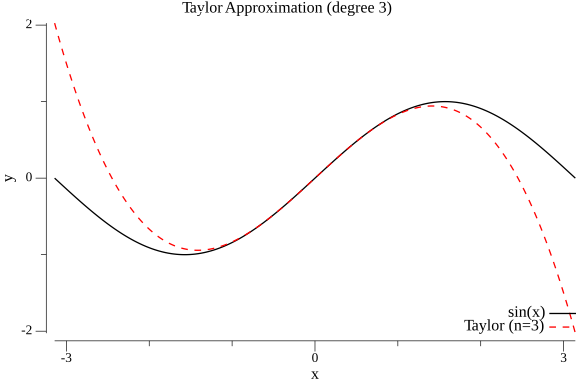
\includegraphics[width=1.0\linewidth]{material/sin/taylor/sin_taylor_n01.png}
  \end{minipage}
  \hfill
  \begin{minipage}[b]{0.48\linewidth}
    \centering
    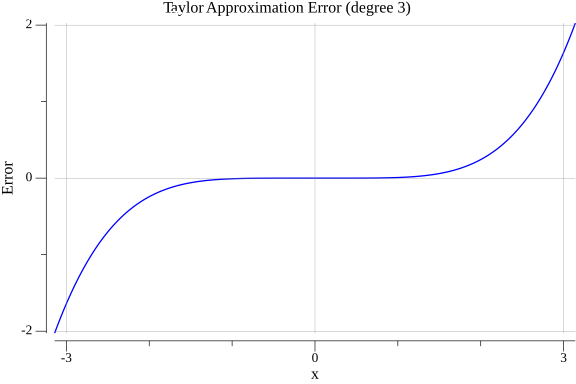
\includegraphics[width=1.0\linewidth]{material/sin/taylor/sin_taylor_err_n01.png}
  \end{minipage}
\end{figure}

\begin{figure}[H]
  \centering
  \caption{$f(x) = \sin(x)$のテイラー展開（11次多項式）}
  \label{fig:sin-taylor-2}
  \vspace{5pt}
  \begin{minipage}[b]{0.48\linewidth}
    \centering
    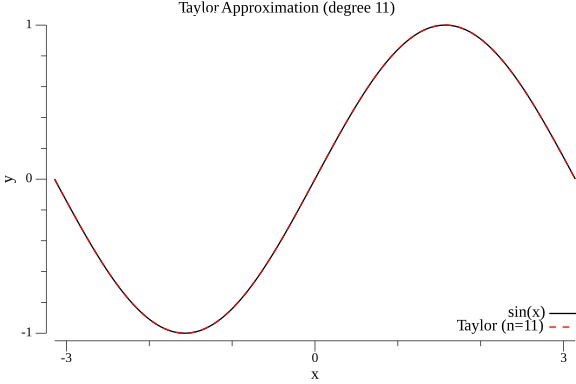
\includegraphics[width=1.0\linewidth]{material/sin/taylor/sin_taylor_n05.png}
  \end{minipage}
  \hfill
  \begin{minipage}[b]{0.48\linewidth}
    \centering
    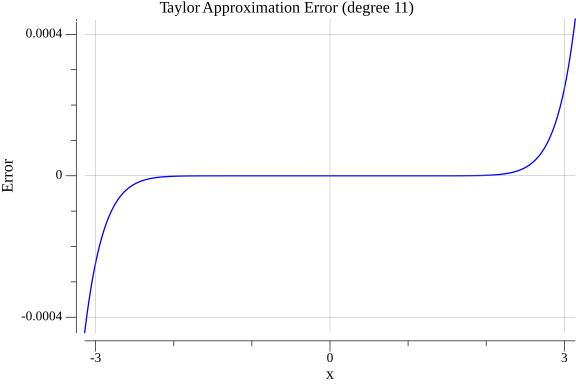
\includegraphics[width=1.0\linewidth]{material/sin/taylor/sin_taylor_err_n05.png}
  \end{minipage}
\end{figure}

\begin{figure}[H]
  \centering
  \caption{$f(x) = \sin(x)$のテイラー展開（23次多項式）}
  \label{fig:sin-taylor-last}
  \vspace{5pt}
  \begin{minipage}[b]{0.48\linewidth}
    \centering
    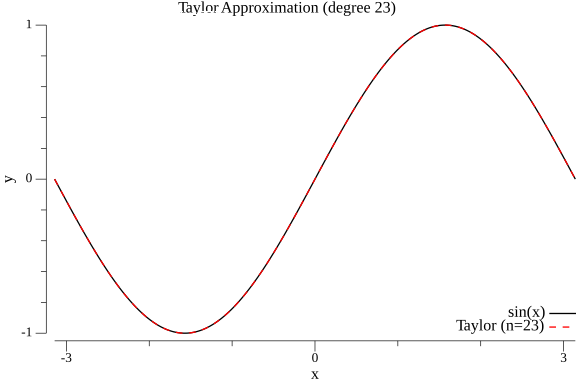
\includegraphics[width=1.0\linewidth]{material/sin/taylor/sin_taylor_n11.png}
  \end{minipage}
  \hfill
  \begin{minipage}[b]{0.48\linewidth}
    \centering
    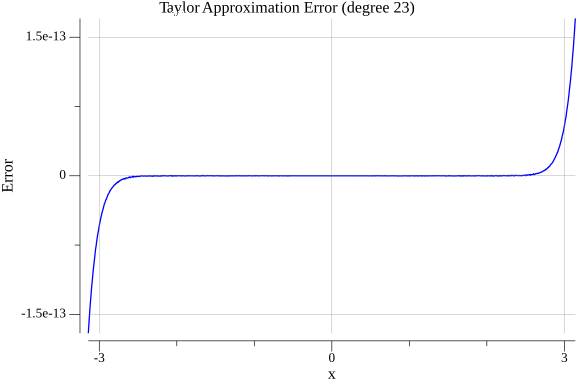
\includegraphics[width=1.0\linewidth]{material/sin/taylor/sin_taylor_err_n11.png}
  \end{minipage}
\end{figure}



    テイラー展開は展開中心点付近では優れた近似性を持つが，
    中心点から遠く離れた領域では精度が低下する傾向がある．
    

  \subsection{ラグランジュ補間多項式による近似：成功例}
    一方，ラグランジュ補間多項式 $p_n(x)$ は，$n+1$個の標本点を補完する多項式を構成する方法である．
    補間多項式の精度は，標本点の選択方法に大きく依存する．
    
    成功例として，$f(x) = \sin(x)$ を $[-\frac{\pi}{2}, \frac{\pi}{2}]$ で補間する場合を考える．
    sin関数は等間隔点による補間でもある程度の精度を得ることができる．
    
    \clearpage
    % =========================================================
    % sin関数による成功例
    % Goプログラム (sin_unified.go) が生成した
    % 等間隔補間の可視化ファイルを読み込む
    % =========================================================
    % sin関数の等間隔補間による比較図

\begin{figure}[H]
  \centering
  \caption{$f(x) = \sin(x)$の等間隔補間（$n=1$次多項式）}
  \label{fig:sin-interp-first}
  \vspace{5pt}
  \begin{minipage}[b]{0.48\linewidth}
    \centering
    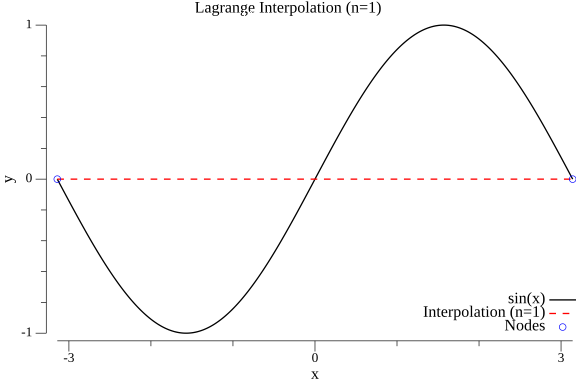
\includegraphics[width=1.0\linewidth]{material/sin/interp/sin_interp_n01.png}
  \end{minipage}
  \hfill
  \begin{minipage}[b]{0.48\linewidth}
    \centering
    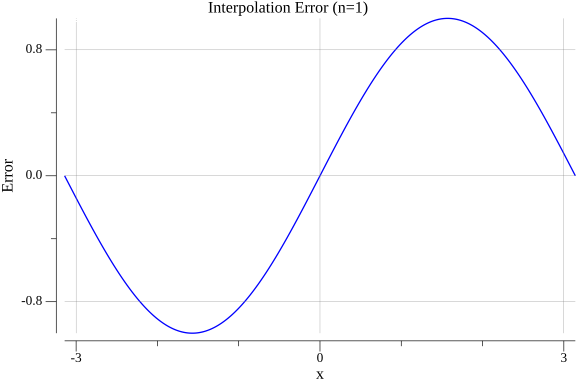
\includegraphics[width=1.0\linewidth]{material/sin/interp/sin_interp_err_n01.png}
  \end{minipage}
\end{figure}

\begin{figure}[H]
  \centering
  \caption{$f(x) = \sin(x)$の等間隔補間（$n=5$次多項式）}
  \label{fig:sin-interp-2}
  \vspace{5pt}
  \begin{minipage}[b]{0.48\linewidth}
    \centering
    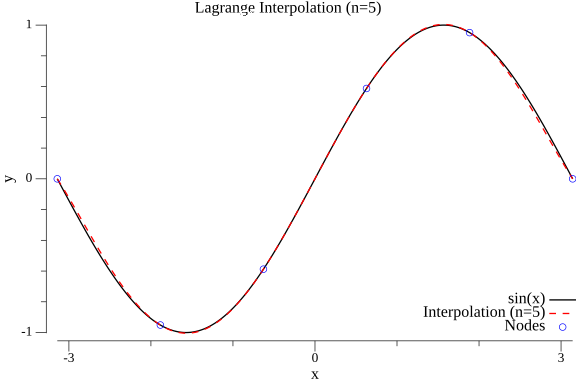
\includegraphics[width=1.0\linewidth]{material/sin/interp/sin_interp_n05.png}
  \end{minipage}
  \hfill
  \begin{minipage}[b]{0.48\linewidth}
    \centering
    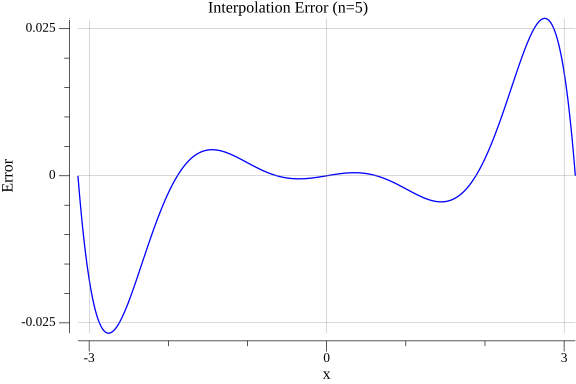
\includegraphics[width=1.0\linewidth]{material/sin/interp/sin_interp_err_n05.png}
  \end{minipage}
\end{figure}

\begin{figure}[H]
  \centering
  \caption{$f(x) = \sin(x)$の等間隔補間（$n=11$次多項式）}
  \label{fig:sin-interp-last}
  \vspace{5pt}
  \begin{minipage}[b]{0.48\linewidth}
    \centering
    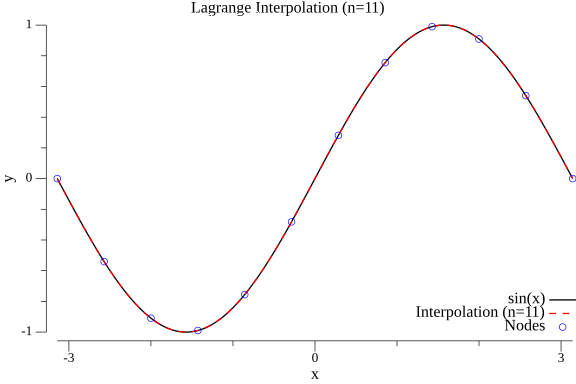
\includegraphics[width=1.0\linewidth]{material/sin/interp/sin_interp_n11.png}
  \end{minipage}
  \hfill
  \begin{minipage}[b]{0.48\linewidth}
    \centering
    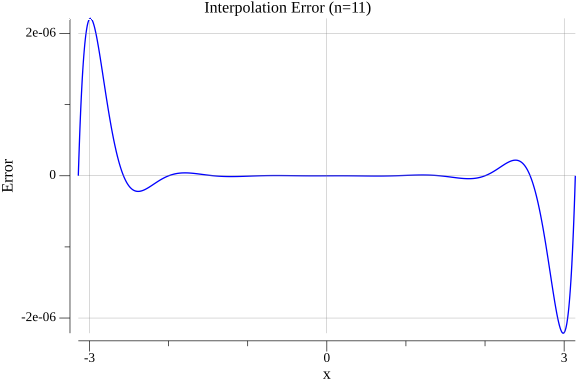
\includegraphics[width=1.0\linewidth]{material/sin/interp/sin_interp_err_n11.png}
  \end{minipage}
\end{figure}


\label{subsec:runge_phenomenon}
  
    このような関数に対しては等間隔点でも良好な近似が得られることが分かる．

  \subsection{ルンゲ現象：等間隔点による補間が失敗する例}
    しかし，すべての関数に対して等間隔点による補間が成功するわけではない．
    代表的な反例として，次の関数を考える．
    \[f(x) = \frac{1}{1 + 25x^2}.\]
    
    この関数は一見すると単純であるが，この式の等間隔標本点の補間多項式は区間の端点付近で急激に変化する特性を持つ．
    この関数に対して等間隔点による補間を行うと，次のように予想外の振動が生じる．
  
    \clearpage  
    % =========================================================
    % Goプログラム (runge_unified.go) が生成した
    % 等間隔補間の可視化ファイルを読み込む
    % =========================================================
    % ルンゲ関数の等間隔補間による比較図

\begin{figure}[H]
  \centering
  \caption{$f(x) = \frac{1}{1+25x^2}$の等間隔補間（$n=4$次多項式）}
  \label{fig:runge-equidistant-first}
  \vspace{5pt}
  \begin{minipage}[b]{0.48\linewidth}
    \centering
    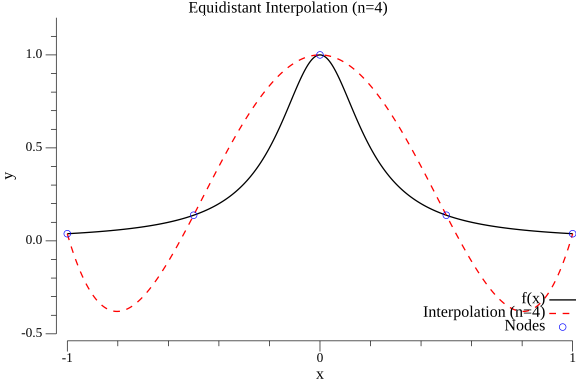
\includegraphics[width=1.0\linewidth]{material/runge/equidistant/runge_n04.png}
  \end{minipage}
  \hfill
  \begin{minipage}[b]{0.48\linewidth}
    \centering
    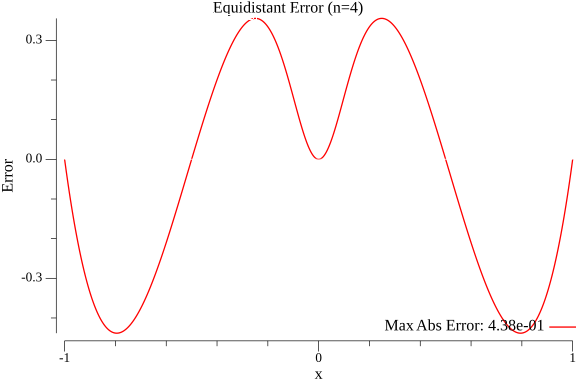
\includegraphics[width=1.0\linewidth]{material/runge/equidistant/runge_err_n04.png}
  \end{minipage}
\end{figure}

\begin{figure}[H]
  \centering
  \caption{$f(x) = \frac{1}{1+25x^2}$の等間隔補間（$n=7$次多項式）}
  \label{fig:runge-equidistant-2}
  \vspace{5pt}
  \begin{minipage}[b]{0.48\linewidth}
    \centering
    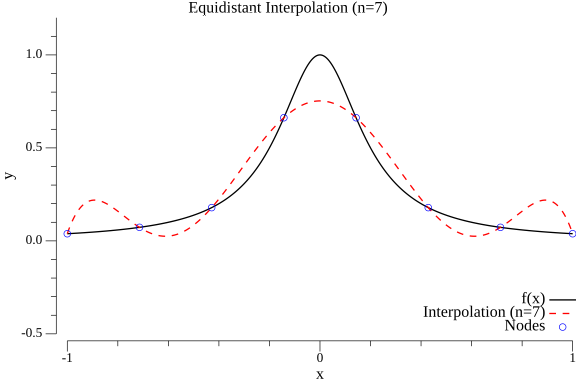
\includegraphics[width=1.0\linewidth]{material/runge/equidistant/runge_n07.png}
  \end{minipage}
  \hfill
  \begin{minipage}[b]{0.48\linewidth}
    \centering
    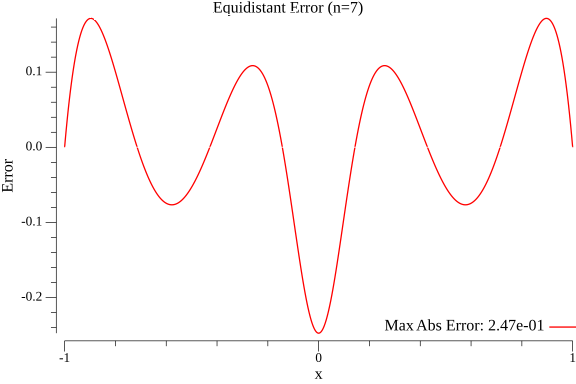
\includegraphics[width=1.0\linewidth]{material/runge/equidistant/runge_err_n07.png}
  \end{minipage}
\end{figure}

\begin{figure}[H]
  \centering
  \caption{$f(x) = \frac{1}{1+25x^2}$の等間隔補間（$n=15$次多項式）}
  \label{fig:runge-equidistant-last}
  \vspace{5pt}
  \begin{minipage}[b]{0.48\linewidth}
    \centering
    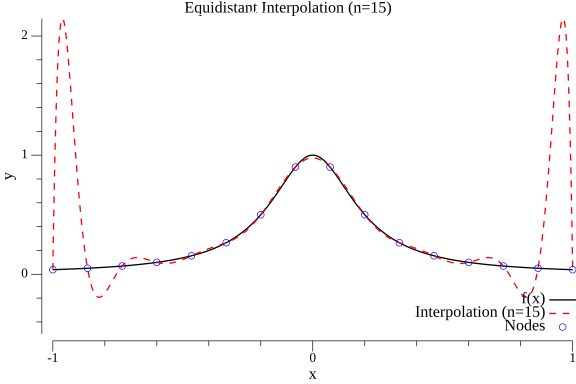
\includegraphics[width=1.0\linewidth]{material/runge/equidistant/runge_n15.png}
  \end{minipage}
  \hfill
  \begin{minipage}[b]{0.48\linewidth}
    \centering
    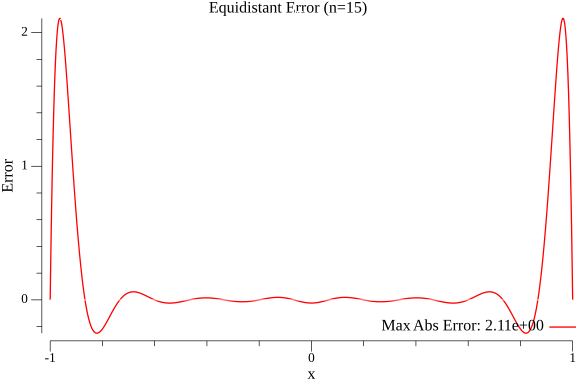
\includegraphics[width=1.0\linewidth]{material/runge/equidistant/runge_err_n15.png}
  \end{minipage}
\end{figure}



  \label{subsec:chebyshev_solution}
    このような現象を\textbf{ルンゲ現象}という．
    多項式の次数を増やしても誤差が減少するどころか，むしろ悪化してしまう場合がある．

  \subsection{チェビシェフ多項式を用いた標本点による補間：失敗例の改善}
    ルンゲ現象を回避するための一つの方法として，振幅が大きくなった端点付近に標本点を集中させる方法がある．
    その手法の一つとして，次のようなチェビシェフ多項式 $T_{n+1}(x)$ の零点を標本点として用いる方法が知られている．
    \begin{equation}
      x_k = \cos \left( \frac{2k + 1}{2(n + 1)} \pi \right) \quad (k = 0, 1, \dots, n).
    \end{equation}
    
    チェビシェフ多項式の零点を用いると，標本点が区間の両端に集中するため，補間多項式の振動が抑制される．
    同じルンゲ関数に対してチェビシェフ多項式の零点を用いた結果は以下の通りである．
    \clearpage
    % =========================================================
    % Goプログラム (runge_unified.go) が生成した
    % チェビシェフ補間の可視化ファイルを読み込む
    % =========================================================
    \input{material/runge/runge_chebyshev_result}

    チェビシェフ多項式の零点を用いた結果（図 \ref{fig:runge-chebyshev-first}～図 \ref{fig:runge-chebyshev-last}）は
    等間隔標本点を採用した結果（図 \ref{fig:runge-equidistant-first}～図 \ref{fig:runge-equidistant-last}）に比べて，振動を大幅に抑制できている．
    ただし，この多項式は標本点を通るだけであり，区間全体における誤差が最も小さい点であるかといわれるとそうではない．
    
    このように，補間多項式の標本点の選択は，補間する関数の性質に大きく依存する重要な要素である．
    次章では最も良い近似を得るためのゴールの一つとして最良近似多項式と呼ばれるものについて述べる．
    最良近似多項式を大まかに説明すると，区間全体における誤差を最小化する多項式である．
\clearpage

% 第2章 最良近似多項式の理論
\section{最良近似多項式の理論} % 二章
\label{sec:best_approximation_theory}
  本章では，連続関数の多項式による最良近似問題について，存在，一意性，および特徴について記述する．
  これらの理論的結果は，次章で述べるRemesのアルゴリズムの正当性を保証するものである．
  なお，本章の議論は主に参考文献\cite{seminar-note}に基づく．

  \subsection{近似度と最良近似の存在}
   \label{subsec:approximation_error}
    関数$f(x)$を多項式$P(x)$で近似する．$f(x)$は有界閉区間[a,b]上で連続関数とする．
    また，$n$ 次以下の多項式全体の集合を $\mathcal{P}_n$ とする．

    \begin{definition}[最良近似多項式]
    \label{def:best_approximation_poly}
    区間 $[a, b]$ 上の連続関数 $f \in C[a, b]$ と，$n$ 次以下の多項式 $P \in \mathcal{P}_n$ に対して，近似度（一様ノルム）を次式で定義する．
    \begin{equation}
      \| f - P\|_\infty = \max_{x \in [a, b]} |f(x) - P(x)|.
      \label{eq:uniform_norm}
    \end{equation}
    さらに，近似誤差の下限を
    \begin{equation}
      E_n(f) = \inf_{P \in \mathcal{P}_n} \| f - P \|_\infty
      \label{eq:best_approx_error}
    \end{equation}
    とおく． このとき，$\| f - P^* \|_\infty = E_n(f)$ を満たす多項式 $P^* \in \mathcal{P}_n$ を，$f$ の $n$ 次最良近似多項式と呼ぶ．
    \end{definition}

    このような多項式 $P^*$ が実際に存在することは，$\mathcal{P}_n$ が有限次元空間であることから示すことができる．

    \begin{theorem}[最良近似多項式の存在]
      \label{thm:existence}
      $[a, b]$における任意の連続関数 $f$ に対して，$n$ 次最良近似多項式 $P^* \in \mathcal{P}_n$ が存在する．
      すなわち,最良近似誤差の下限を達成する$P^* \in \mathcal{P}_n$ が存在する
      ．
    \end{theorem}

    \begin{proof}
      下限の定義（式 \ref{eq:best_approx_error}）より，近似誤差が下限値 $E_n(f)$ に収束するような$n$次多項式の列 $\{P^{(\nu)}\}_{\nu=1}^\infty$が存在する． すなわち，
      \[ \lim_{\nu \to \infty} \| f - P_\nu \|_\infty = E_n(f) \]
      である． このとき，三角不等式により
      \begin{equation}
        \| P_\nu \|_\infty \le \| f - P_\nu \|_\infty + \| f \|_\infty
      \end{equation}
      が成り立つ． 十分大きな $\nu$ に対して $\| f - P_\nu \|_\infty \le E_n(f) + 1$ と評価できるため，
      \[ \| P_\nu \|_\infty \le E_n(f) + 1 + \| f \|_\infty \]
      となり，列 $\{P_\nu\}$ は一様有界である．
      $\mathcal{P}_n$ は有限次元ベクトル空間（$\mathbb{R}^{n+1}$ と同型）であるため，ボルツァーノ・ワイエルシュトラスの定理（またはハイネ・ボレルの被覆定理）より，$\{P_\nu\}$ は収束する部分列 $\{P_{\nu_k}\}$ を持つ．
      その極限を $P^* = \lim_{k \to \infty} P_{\nu_k} \in \mathcal{P}_n$ とすれば，ノルムの連続性より
      \begin{equation}
        \| f - P^* \|_\infty = \lim_{k \to \infty} \| f - P_{\nu_k} \|_\infty = E_n(f)
      \end{equation}
      となり，$P^*$ が求める最良近似多項式であることが示される．
    \end{proof}

  \subsection{近似誤差の下限評価}
    \label{subsec:lower_bound_error}
    最良近似多項式の特徴付けを行う準備として，近似誤差の下限評価を与える補題を用意する．
    まず，誤差関数の符号が交互に変化するような点列（交代点列）を定義する．
    \begin{definition}[交代点列]
    \label{def:alternation_points}
      
      区間 $[a, b]$ 内の狭義単調増加列 $a \le \xi_0 < \xi_1 < \dots < \xi_{r-1} \le b$ に対して，誤差 $f(\xi_i) - P(\xi_i)$ が交互に符号を変えるとき，$\xi = (\xi_0, \dots, \xi_{r-1})$ を長さ $r$ の交代点列と呼ぶ．
      長さ $r$ の交代点列全体を $\Xi_r(f, P)$ と表す．すなわち，
      \begin{equation}
        \begin{split}
          \Xi_r(f, P) = \{ \xi = (\xi_0, \dots, \xi_{r-1}) \mid & a \le \xi_0 < \dots < \xi_{r-1} \le b, \ \\
          & (f(\xi_i) - P(\xi_i)) \cdot (f(\xi_{i+1}) - P(\xi_{i+1})) < 0 \}
        \end{split}
      \end{equation}
      である．さらに，この点列上での最小誤差を
      \begin{equation}
        \Phi(f, P, \xi) = \min_{0 \le i \le r-1} |f(\xi_i) - P(\xi_i)|
      \end{equation}
    \end{definition}
    \noindent
    と定義する．
    
    すると，以下の評価が成り立つ．

    \begin{lemma}
      \label{lem:lower_bound}
      $P \in \mathcal{P}_n$ とし，$\xi \in \Xi_{n+2}(f, P)$ ならば，
      \begin{equation}
        \Phi(f, P, \xi) \le E_n(f)
      \end{equation}
      が成り立つ．
    \end{lemma}

    \begin{proof}
      背理法で示す．不等式が成り立たない，すなわち $E_n(f) < \Phi(f, P, \xi)$ と仮定する．
      このとき，定理\ref{thm:existence}より，ある $\tilde{P} \in \mathcal{P}_n$ が存在して
      \begin{equation}
        \| f - \tilde{P} \|_\infty < \Phi(f, P, \xi)
      \end{equation}
      を満たす．ここで，差 $P(x) - \tilde{P}(x)$ を考えると，
      \begin{equation}
        P(\xi_i) - \tilde{P}(\xi_i) = (f(\xi_i) - \tilde{P}(\xi_i)) - (f(\xi_i) - P(\xi_i)) \label{eq:best_approx_error}
      \end{equation}
      である．仮定より
      \begin{equation}
      |f(\xi_i) - \tilde{P}(\xi_i)| \le \| f - \tilde{P} \|_\infty < \Phi(f, P, \xi) \le |f(\xi_i) - P(\xi_i)|
      \end{equation}
      であるため，\eqref{eq:best_approx_error} の符号は右辺の第2項 $-(f(\xi_i) - P(\xi_i))$ の符号に依存している．
      
      $\xi \in \Xi_{n+2}(f, P)$ より $f(\xi_i) - P(\xi_i)$ の符号は交互に入れ替わるため，$P(\xi_i) - \tilde{P}(\xi_i)$ の符号も交互に入れ替わる．
      したがって，連続関数の符号の交代性から（中間値の定理） $P(x) - \tilde{P}(x)$ は各区間 $(\xi_i, \xi_{i+1})$ に少なくとも1つの零点を持つ．
      点は $n+2$ 個あるため区間は $n+1$ 個あり，$P - \tilde{P}$ は少なくとも $n+1$ 個の零点を持つことになる．
      $P - \tilde{P} \in \mathcal{P}_n$ であるため，これが $n+1$ 個の零点を持つならば $P = \tilde{P}$ でなければならない．
      すると $\| f - P \|_\infty < \Phi(f, P, \xi) \le \| f - P \|_\infty$ となり矛盾する．
    \end{proof}

  \label{subsec:alternation_theorem}
  \subsection{チェビシェフの交代定理}

    最良近似多項式の必要十分条件を与えるのが，以下の交代定理である．
    この定理は，Remesアルゴリズムの収束判定条件として本研究の根幹をなすものである．

    \begin{theorem}[交代定理]

      \label{thm:koutaiteiri}
      $f \in C[a, b]$ に対し，$P^* \in \mathcal{P}_n$ が最良近似多項式であるための必要十分条件は，長さ $n+2$ の交代偏差点列 $\xi \in \Xi_{n+2}(f, P^*)$ が存在することである．
      ここで交代偏差点列とは，各点 $\xi_i$ が偏差点（誤差が最大ノルムを達成する点），すなわち
      \begin{equation}
        |f(\xi_i) - P^*(\xi_i)| = \|f - P^*\|_\infty
      \end{equation}
      を満たすような交代点列のことである．
    \end{theorem}

    \begin{proof}
      \textbf{（十分性）}
      長さ $n+2$ の交代偏差点列 $\xi \in \Xi_{n+2}(f, P^*)$ が存在すると仮定する．
      このとき， $\Phi(f, P^*, \xi)$ の定義\ref{def:alternation_points}より
      \[ \Phi(f, P^*, \xi) = \min_{i} |f(\xi_i) - P^*(\xi_i)| = \|f - P^*\|_\infty \]
      である． 補題\ref{lem:lower_bound}より，一般に $\Phi(f, P^*, \xi) \le E_n(f)$ が成り立つため，
      \begin{equation}
        \|f - P^*\|_\infty \le E_n(f)
      \end{equation}
      となる． 一方，最良近似誤差の定義\ref{def:best_approximation_poly}より $E_n(f) \le \|f - P^*\|_\infty$ は常に成り立つため，
      \[ \|f - P^*\|_\infty = E_n(f) \]
      となり，$P^*$ は最良近似多項式であることが示される．

      \textbf{（必要性）}
      背理法により示す． $P^*$ が最良近似多項式であるにもかかわらず，交代偏差点列の長さが $n+2$ 未満であると仮定する．
      すなわち，存在する交代偏差点列の中で点の個数が最大となるものを選び，それを $\xi_0 < \xi_1 < \dots < \xi_m$ とおく．このとき，仮定より $m+1 \le n+1$ である．
      
      このとき，誤差関数 $e(x) = f(x) - P^*(x)$ の符号変化を利用して，最大誤差ノルムを減少させる多項式が存在することを示し，$P^*$ が最良近似多項式であることと矛盾することを導く．

      まず，隣り合う偏差点 $\xi_{i-1}, \xi_i$ の間で，誤差関数の符号が変化する点（零点）を $t_i$ ($i=1, \dots, m$) として選ぶことができる．ここで，補正のための多項式 $K(x)$ を次のように定義する．
      \begin{equation}
        K(x) = \prod_{i=1}^m (t_i - x).
        \label{eq:correction_poly}
      \end{equation}
      仮定より $m \le n$ であるため，$K(x)$ の次数は $n$ 以下であり，$K \in \mathcal{P}_n$ である．
      この $K(x)$ は，各区間 $(t_i, t_{i+1})$ において符号が一定であり，その符号変化のパターンは誤差関数 $e(x)$ と一致する．
      ここで，偏差点 $\xi_i$ における符号を合わせるために，$\sigma = \text{sgn}(e(\xi_0) K(\xi_0))$ とおく．

      今，正の定数 $\lambda > 0$ を用いて新しい多項式 $P_\lambda(x) = P^*(x) + \lambda \sigma K(x)$ を考えると，その誤差は
      \[ f(x) - P_\lambda(x) = (f(x) - P^*(x)) - \lambda \sigma K(x) = e(x) - \lambda \sigma K(x) \]
      となる．
      偏差点 $\xi_i$ を含む近傍では，$e(x)$ と $\sigma K(x)$ が同符号であるため，適切な $\lambda$ を選んで $\lambda \sigma K(x)$ を引くことで，誤差の絶対値 $|e(x)|$ を減少させることができる．      
      一方，偏差点以外の場所では誤差が増大する可能性があるが，$\lambda$ を十分に小さくとることで，増大分を抑え込み，全体として
      \begin{equation}
        \| f - P_\lambda \|_\infty < \| f - P^* \|_\infty
      \end{equation}
      を満たすようにできる．
      これは $P^*$ が最良近似多項式であること（誤差ノルムが最小であること）に矛盾する．
      したがって，最良近似多項式が存在するならば，交代偏差点列の長さは $n+2$ 以上でなければならない．
    \end{proof}
  \label{subsec:uniqueness}
    
  \subsection{一意性}
    \begin{theorem}[最良近似多項式の一意性]
    \label{thm:uniqueness}
      連続関数 $f \in C[a, b]$ に対する $n$ 次最良近似多項式 $P^*$ は一意に定まる．
    \end{theorem}

    \begin{proof}
      背理法により示す． $P^*_1, P^*_2 \in \mathcal{P}_n$ が共に $f$ の最良近似多項式であり，$P^*_1 \neq P^*_2$ であると仮定する．
      このとき，最良近似誤差は $E_n(f) = \|f - P^*_1\|_\infty = \|f - P^*_2\|_\infty$ である．
      ここで，これら2つの多項式の平均 $P_{avg} = \frac{1}{2}(P^*_1 + P^*_2)$ を考えると，三角不等式より
      \begin{equation}
        \|f - P_{avg}\|_\infty = \left\| \frac{1}{2}(f - P^*_1) + \frac{1}{2}(f - P^*_2) \right\|_\infty
        \le \frac{1}{2}\|f - P^*_1\|_\infty + \frac{1}{2}\|f - P^*_2\|_\infty = E_n(f)
      \end{equation}
      が成り立つ． 一方，$E_n(f)$ は誤差の下限であるため $\|f - P_{avg}\|_\infty \ge E_n(f)$ である．
      したがって $\|f - P_{avg}\|_\infty = E_n(f)$ となり，$P_{avg}$ もまた最良近似多項式であることがわかる．

      $P_{avg}$ は最良近似多項式であるため，定理 \ref{thm:koutaiteiri}（交代定理）より，長さ $n+2$ の交代偏差点列 $\xi \in \Xi_{n+2}(f, P_{avg})$ が存在する．
      すなわち，ある符号 $\sigma \in \{1, -1\}$ を用いて，各点 $\xi_i$ ($i=0, \dots, n+1$) において以下が成り立つ．
      \begin{equation}
        f(\xi_i) - P_{avg}(\xi_i) = \sigma (-1)^i E_n(f).
      \end{equation}
      この式の左辺に $P_{avg} = \frac{1}{2}(P^*_1 + P^*_2)$ を代入して変形すると，
      \begin{equation}
        \frac{1}{2}(f(\xi_i) - P^*_1(\xi_i)) + \frac{1}{2}(f(\xi_i) - P^*_2(\xi_i)) = \sigma (-1)^i E_n(f)
        \label{eq:uniq_sum}
      \end{equation}
      となる． ここで，$P^*_1, P^*_2$ は最良近似多項式であるため，任意の点での誤差の絶対値は $E_n(f)$ 以下である．
      すなわち，
      \[ |f(\xi_i) - P^*_1(\xi_i)| \le E_n(f), \quad |f(\xi_i) - P^*_2(\xi_i)| \le E_n(f) \]
      である．
      式 (\ref{eq:uniq_sum}) は，「絶対値が $E_n(f)$ 以下の2つの実数の平均が，ちょうど境界値 $\pm E_n(f)$ になっている」ことを意味する．
      これが成り立つのは，2つの実数が共に境界値と等しい場合のみである．
      したがって，すべての $i=0, \dots, n+1$ において
      \begin{equation}
        f(\xi_i) - P^*_1(\xi_i) = f(\xi_i) - P^*_2(\xi_i) = \sigma (-1)^i E_n(f)
      \end{equation}
      が成立しなければならない． よって
      \[ P^*_1(\xi_i) = P^*_2(\xi_i) \quad (i = 0, 1, \dots, n+1) \]
      となり，2つの $n$ 次多項式が異なる $n+2$ 個の点で一致することになる．
      $n$ 次多項式が $n+1$ 個以上の点で一致すれば恒等的に等しいため，$P^*_1 = P^*_2$ となり，仮定に矛盾する．
      ゆえに最良近似多項式は一意に定まる．
    \end{proof}


\newpage  %% 改ページ ==================================================

% 第3章 Remesアルゴリズムによる最良近似多項式の計算
\section{Remesアルゴリズムによる最良近似多項式の計算}
\label{sec:remes_algorithm}

本章では，第2章で述べた最良近似多項式の存在定理および交替定理に基づき，実際に最良近似多項式を数値的に求めるためのアルゴリズムであるRemesアルゴリズムについて説明する．
このアルゴリズムは，1934年にEvgeny Remesによって提案された反復解法であり，任意の連続関数に対して，交替定理の条件を満たす参照点を効率的に探索する手法である．

\subsection{アルゴリズムの概要と計算手順}
\label{subsec:algo_overview}

Remesアルゴリズムの基本的なアイデアは，区間 $[a, b]$ 内の $n+2$ 個の参照点 $\xi^{(k)} = \{x_0^{(k)}, x_1^{(k)}, \dots, x_{n+1}^{(k)}\}$ を初期設定し，反復ごとにこれを更新して，最終的に誤差関数の極値点と参照点が一致するように収束させることである．
特に，本研究では収束速度に優れる「全点同時入れ替え法」を採用する．

アルゴリズムの各ステップは以下の通りである．

\subsubsection{Step 0: 初期参照点の設定}
近似区間 $[a, b]$ 内に，$a \le x_0 < x_1 < \dots < x_{n+1} \le b$ を満たす $n+2$ 個の点を選び，初期参照点 $\xi^{(0)}$ とする．
初期値の選び方は任意であるが，収束を速めるために，通常はチェビシェフ多項式の極値点を区間 $[a, b]$ に写像した点が用いられる．

\subsubsection{Step 1: 近似多項式の導出（係数決定）}
現在の参照点 $\boldsymbol{\xi}^{(k)}$ 上で，誤差が交互に符号を変え，かつその絶対値が等しくなるような多項式 $P(x)$ と，その誤差の大きさ $E$ を決定する．
この $E$ は，現在の参照点集合 $\boldsymbol{\xi}^{(k)}$ の上でのみ成立する均等な誤差であり，これを\textbf{参照均等誤差}（levelled reference error）と呼ぶ\cite{seminar-note}．
具体的には，以下の連立方程式を解く．

\begin{equation}
    f(\xi_i) - P(\xi_i) = (-1)^i E \quad (i = 0, 1, \dots, n+1).
    \label{eq:remes_linear_system}
\end{equation}

ここで，$P(\xi) = \sum_{j=0}^n c_j \xi^j$ とおくと，式(\ref{eq:remes_linear_system})は係数 $c_0, \dots, c_n$ および $E$ を未知数とする $n+2$ 元の連立一次方程式となる．
これを行列形式で記述すると以下のようになる．

\begin{equation}
    \left(
    \begin{array}{ccccc}
    1 & \xi_0 & \dots & \xi_0^n & 1 \\
    1 & \xi_1 & \dots & \xi_1^n & -1 \\
    \vdots & \vdots & \ddots & \vdots & \vdots \\
    1 & \xi_{n+1} & \dots & \xi_{n+1}^n & (-1)^{n+1}
    \end{array}
    \right)
    \left(
    \begin{array}{c}
    c_0 \\
    c_1 \\
    \vdots \\
    c_n \\
    E
    \end{array}
    \right)
    =
    \left(
    \begin{array}{c}
    f(\xi_0) \\
    f(\xi_1) \\
    \vdots \\
    f(\xi_{n+1})
    \end{array}
    \right).
\end{equation}

この方程式をLU分解で解くことで，現在の参照点集合に対する「最良近似」となる多項式 $P(x)$ が一意に定まる．

\subsubsection{Step 2: 誤差関数の極値探索}
求めた多項式 $P(x)$ に対する誤差関数 $e(x) = f(x) - P(x)$ を定義し，区間 $[a, b]$ 全体における極値を探索する．
具体的には，$e(x)$ の極大値・極小値を与える点，および区間の端点の中から，誤差の絶対値 $|e(x)|$ が現在の均等誤差 $|E|$ よりも大きくなる点を探し出す．

もし，すべての $x \in [a, b]$ において $|e(x)| \le |E| + \varepsilon$ （$\varepsilon$ は許容誤差）が成り立つならば，現在の $P(x)$ は最良近似多項式であるとみなしてアルゴリズムを終了する．

\subsubsection{Step 3: 参照点の更新（全点同時入れ替え）}
Step 2 で見つけた極値点を用いて，次の参照点 $\xi^{(k+1)}$ を決定する．
新しい参照点集合は，交替定理の条件（誤差の符号が交互になること）を維持しつつ，各点での誤差の絶対値ができるだけ大きくなるように選ばれる．

一般的には，誤差関数 $e(x)$ の零点を境界として区間を分割し，各部分区間内で $|e(x)|$ が最大となる点を新しい参照点 $x_i^{(k+1)}$ として採用する．
これにより，参照点は真の最良近似における極値点へと近づいていく．

\subsection{Remesアルゴリズムの収束性}
\label{subsec:remes_convergence}
対象関数 $f(x)$ が区間 $[a, b]$ 上で十分に滑らか（$C^2$級以上）であり，かつ最良近似多項式の誤差関数が正常な数（ちょうど $n+2$ 個）の極値を持つ場合，
全点同時入れ替え法を用いたRemesアルゴリズムは2次収束することが知られている．
本節では，このアルゴリズムがニュートン法によってそれが保証される事を示し，その収束性を理論的に説明する．
なお，本節の議論は参考文献\cite{seminar-note}に基づく．

\subsubsection{最良近似問題の非線形方程式への帰着}

対象関数 $f(x)$ が区間 $[a, b]$ 上で2回連続微分可能であり，その最良近似多項式 $P^*(x)$ の誤差関数 $e^*(x) = f(x) - P^*(x)$ が，区間内部にちょうど $n+1$ 個の極値を持つ（端点を含めて $n+2$ 個の偏差点を持つ）と仮定する．

このとき，最良近似多項式を決定するために求めるべき未知数は，以下の3組である．
\begin{itemize}
  \item 多項式の係数ベクトル $\boldsymbol{c} = (c_0, \dots, c_n)$ \quad ($n+1$ 個)
  \item 最大誤差（均等誤差） $E$ \quad ($1$ 個)
  \item 偏差点列の座標ベクトル $\boldsymbol{\xi} = (\xi_0, \dots, \xi_{n+1})$ \quad ($n+2$ 個)
\end{itemize}
これら合計 $2n+4$ 個の変数は，以下の連立非線形方程式の解として特徴づけられる．

\begin{numcases}{}
  f(\xi_i) - \sum_{j=0}^n c_j \xi_i^j - (-1)^i E = 0 & $(i = 0, \dots, n+1).$ \label{eq:remes_nonlinear_1} \\
  f'(\xi_i) - \sum_{j=0}^n c_j j \xi_i^{j-1} = 0 & $(i = 1, \dots, n).$ \label{eq:remes_nonlinear_2}
\end{numcases}

式(\ref{eq:remes_nonlinear_1})は交替定理の条件（各点での誤差が $\pm E$ になること）を表し，式(\ref{eq:remes_nonlinear_2})は各点 $\xi_i$ が誤差関数の極値（微分係数が0）であることを表している（端点は固定とする）．

\subsubsection{Remesアルゴリズムとニュートン法との等価性と2次収束性}
\label{subsec:newton_equivalence}

Remesアルゴリズム（全点同時入れ替え法）の反復手順は，前節で導出した非線形方程式系 $\boldsymbol{F}(\boldsymbol{y}) = \boldsymbol{0}$ に対するニュートン法と構造的な対応関係にある．
具体的には，未知数ベクトル $\boldsymbol{y}$ の更新量 $\Delta \boldsymbol{y} = \boldsymbol{y}^{(k+1)} - \boldsymbol{y}^{(k)}$ は，ニュートン法の方程式
\begin{equation}
  \boldsymbol{J}(\boldsymbol{y}^{(k)}) \Delta \boldsymbol{y} = -\boldsymbol{F}(\boldsymbol{y}^{(k)})
  \label{eq:newton_step}
\end{equation}
によって決定されるが，Remesアルゴリズムはこれを以下の2段階に分離して実行していると解釈できる\cite{seminar-note}．

\begin{enumerate}
  \item \textbf{係数と誤差の更新（Step 1に対応）:}
  ニュートン法における係数ベクトル $\boldsymbol{c}$ および $E$ の更新は，方程式系(\ref{eq:remes_nonlinear_1})の線形部分を解くことに相当する．Remesアルゴリズムでは，現在の点 $\boldsymbol{\xi}^{(k)}$ を固定した状態でこの線形方程式を解いている．
  
  \item \textbf{偏差点の更新（Step 2に対応）:}
  偏差点 $\boldsymbol{\xi}$ の更新は，方程式系(\ref{eq:remes_nonlinear_2})すなわち誤差関数の導関数 $e'(x)=0$ の根を求めることに対応する．
  Remesアルゴリズムにおいて，現在の近似多項式 $P^{(k)}$ に基づいて新たな極値を探す操作は，幾何学的には誤差関数の勾配情報を用いた修正を行うことと同義であり，これはニュートン法における $\boldsymbol{\xi}$ 成分の更新ステップ
  \[ \xi_i^{(k+1)} \approx \xi_i^{(k)} - \frac{e'(\xi_i^{(k)})}{e''(\xi_i^{(k)})} \]
  を（高精度な探索によって）実行していることと等価である．
\end{enumerate}

参考文献\cite{seminar-note}によると，解の十分近傍において，このRemesアルゴリズムの手順はニュートン法の反復ステップと（高次の微小項を除いて）一致することが解析的に示されている．

ニュートン法は解の近傍において2次収束することが知られているため，Remesアルゴリズムにおいても，初期参照点 $\boldsymbol{\xi}^{(0)}$ が真の解 $\boldsymbol{\xi}^*$ に十分近ければ，誤差 $\delta_k = \|\boldsymbol{\xi}^{(k)} - \boldsymbol{\xi}^*\|$ は以下の不等式を満たす．

\begin{equation}
  \delta_{k+1} \le C \delta_k^2
\end{equation}

ここで $C$ は正の定数である．
すなわち，解の近傍では誤差が反復ごとに二乗で減少するため，収束が著しく高速となる．

\label{subsec:algo_implementation}
\subsection{アルゴリズムの実装と検証}
% =========================================================
% Goプログラム (remes_comparison.go) が生成した
% プロセス可視化ファイル（グラフと表）を読み込む
% =========================================================
%% 3章用 (Grid)

前述の理論に基づき，本研究ではGo言語を用いてRemesアルゴリズムを実装した．
以下の図表は，関数 $f(x) = \frac{1}{1+25x^2}$ ($n=15$) を近似した際の収束過程を示したものである．

表\ref{tab:remes-grid-log}は，各反復で算出された参照均等誤差 $|E|$ と，その時点での誤差関数の極値の絶対値の最大値と最小値の差（Deviation）の推移を示したものである．

本実装における収束判定条件は，すべてのパラメータの変化量が機械イプシロン（$\epsilon_{\text{mach}} \approx 2.22 \times 10^{-16}$）以下になった時点とする．
\begin{itemize}
  \item 近似多項式の係数ベクトル $\boldsymbol{c}$ の最大変化量：
  \[ \|\boldsymbol{c}^{(k+1)} - \boldsymbol{c}^{(k)}\|_\infty \le \epsilon_{\text{mach}}. \]
  \item 参照点ベクトル $\boldsymbol{\xi}$ の最大変化量：
  \[ \|\boldsymbol{\xi}^{(k+1)} - \boldsymbol{\xi}^{(k)}\|_\infty \le \epsilon_{\text{mach}}. \]
  \item 均等誤差パラメータ $E$ の変化量：
  \[ |E^{(k+1)} - E^{(k)}| \le \epsilon_{\text{mach}}. \]
\end{itemize}
これにより，数値計算上の限界精度まで解が収束したことを保証する．

表中の Deviation は，係数が収束に向かうにつれて交替定理の条件（等振幅性）が満たされていく様子を表す指標であり，理論通り急速に 0 に収束していることが確認できる．

図\ref{fig:remes-grid-convergence}は，この Deviation の推移を可視化したものである．
初期段階では不揃いであった誤差の波形が，最終的には振幅が一定の美しい等振動波形へと収束していることが見て取れる．

\begin{figure}[H]
 \centering
 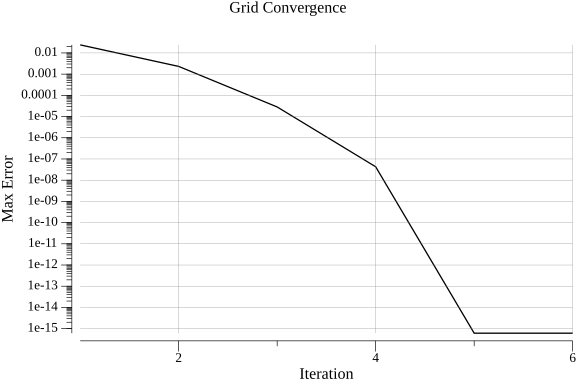
\includegraphics[width=0.6\linewidth]{material/remes/outputs/grid/convergence_grid.png}
 \caption{グリッド極値点探索法による最大誤差の収束履歴}
 \label{fig:remes-grid-convergence}
\end{figure}

\begin{figure}[H]
 \centering
 \begin{minipage}[b]{0.48\textwidth}
  \centering
  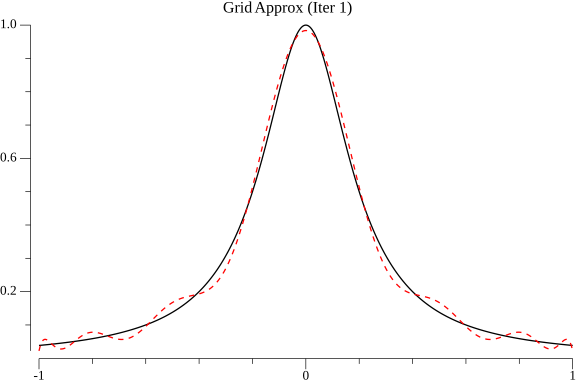
\includegraphics[width=1.0\linewidth]{material/remes/outputs/grid/func_remes_grid_iter01.png}
  \caption{Iter 1}
 \end{minipage}
 \hfill
 \begin{minipage}[b]{0.48\textwidth}
  \centering
  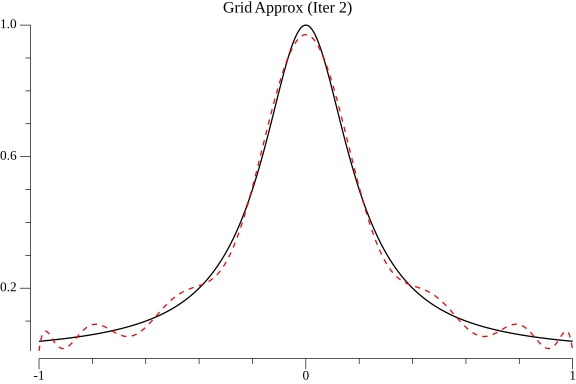
\includegraphics[width=1.0\linewidth]{material/remes/outputs/grid/func_remes_grid_iter02.png}
  \caption{Iter 2}
 \end{minipage}

 \begin{minipage}[b]{0.48\textwidth}
  \centering
  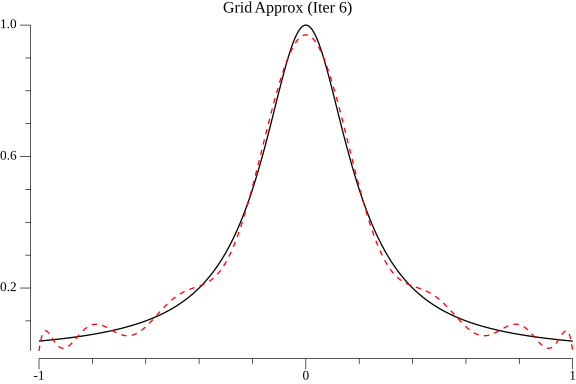
\includegraphics[width=1.0\linewidth]{material/remes/outputs/grid/func_remes_grid_iter06.png}
  \caption{Iter 6}
 \end{minipage}

 \caption{グリッド法: 近似多項式の推移}
 \label{fig:remes-grid-approx}
\end{figure}
\begin{figure}[H]
 \centering
 \begin{minipage}[b]{0.48\textwidth}
  \centering
  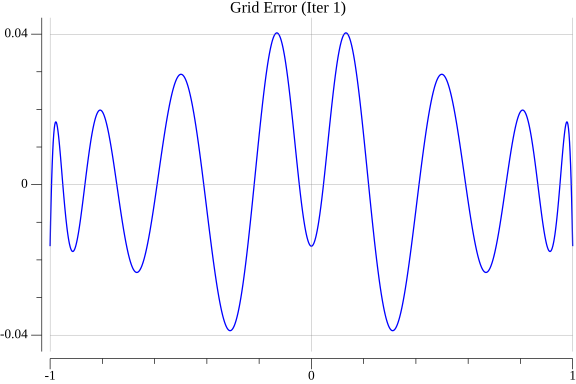
\includegraphics[width=1.0\linewidth]{material/remes/outputs/grid/error_remes_grid_iter01.png}
  \caption{Iter 1}
 \end{minipage}
 \hfill
 \begin{minipage}[b]{0.48\textwidth}
  \centering
  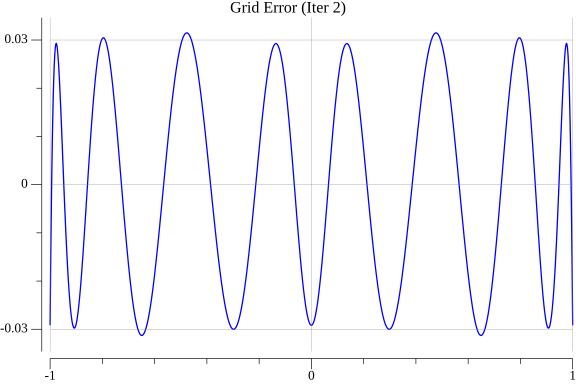
\includegraphics[width=1.0\linewidth]{material/remes/outputs/grid/error_remes_grid_iter02.png}
  \caption{Iter 2}
 \end{minipage}

 \begin{minipage}[b]{0.48\textwidth}
  \centering
  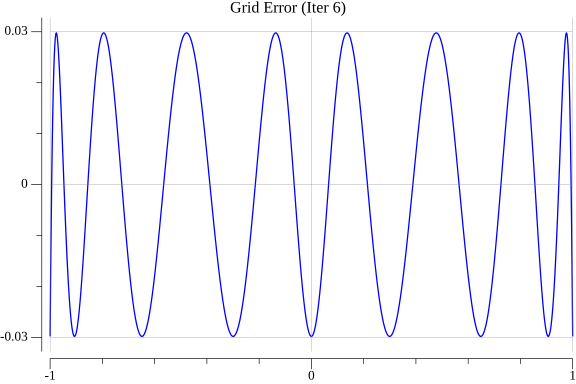
\includegraphics[width=1.0\linewidth]{material/remes/outputs/grid/error_remes_grid_iter06.png}
  \caption{Iter 6}
 \end{minipage}

 \caption{グリッド法: 誤差関数の推移}
 \label{fig:remes-grid-error}
\end{figure}

\begin{table}[H]
 \centering
 \caption{グリッド極値点探索法の収束ログ}
 \label{tab:remes-grid-log}
 \begin{tabular}{crrrr}
 \toprule
 Iter & $|E|$ & Coeff Norm & Node Move & Error Change \\
 \midrule
 1 & $1.63552e-02$ & $0.00000e+00$ & $0.00000e+00$ & $0.00000e+00$ \\
 2 & $2.91689e-02$ & $1.37847e-02$ & $4.92138e-02$ & $1.28137e-02$ \\
 3 & $2.97722e-02$ & $1.25091e-03$ & $3.16228e-03$ & $6.03335e-04$ \\
 4 & $2.97756e-02$ & $1.30728e-05$ & $1.41421e-03$ & $3.38844e-06$ \\
 5 & $2.97756e-02$ & $1.90384e-08$ & $0.00000e+00$ & $7.83719e-09$ \\
 6 & $2.97756e-02$ & $0.00000e+00$ & $0.00000e+00$ & $0.00000e+00$ \\
 \bottomrule
 \end{tabular}
\end{table}

\begin{table}[H]
 \centering
 \caption{グリッド極値点探索結果の等振幅性確認（節点近傍の偏差）}
 \label{tab:remes-grid-final-check}
 \begin{tabular}{crrr}
 \toprule
 No. & Grid誤差 & Brent誤差 & 差分 \\
 \midrule
 1 & $2.97755952e-02$ & $2.97755952e-02$ & $-6.86950e-16$ \\
 2 & $2.97755952e-02$ & $2.97755952e-02$ & $3.80066e-11$ \\
 3 & $2.97755952e-02$ & $2.97755952e-02$ & $1.63316e-11$ \\
 4 & $2.97755952e-02$ & $2.97755952e-02$ & $1.94925e-12$ \\
 5 & $2.97755952e-02$ & $2.97755952e-02$ & $4.93021e-12$ \\
 6 & $2.97755952e-02$ & $2.97755952e-02$ & $1.21936e-12$ \\
 7 & $2.97755952e-02$ & $2.97755952e-02$ & $4.76352e-12$ \\
 8 & $2.97755952e-02$ & $2.97755952e-02$ & $6.46216e-12$ \\
 9 & $2.97755952e-02$ & $2.97755952e-02$ & $0.00000e+00$ \\
 10 & $2.97755952e-02$ & $2.97755952e-02$ & $6.46216e-12$ \\
 11 & $2.97755952e-02$ & $2.97755952e-02$ & $4.76358e-12$ \\
 12 & $2.97755952e-02$ & $2.97755952e-02$ & $1.21927e-12$ \\
 13 & $2.97755952e-02$ & $2.97755952e-02$ & $4.93020e-12$ \\
 14 & $2.97755952e-02$ & $2.97755952e-02$ & $1.94927e-12$ \\
 15 & $2.97755952e-02$ & $2.97755952e-02$ & $1.63316e-11$ \\
 16 & $2.97755952e-02$ & $2.97755952e-02$ & $3.80066e-11$ \\
 17 & $2.97755952e-02$ & $2.97755952e-02$ & $-1.34615e-15$ \\
 \bottomrule
 \end{tabular}
\vspace{1mm}

\small \textbf{注：}
\small 上表は，区間 $[-1.0,1.0]$ を探索するRemesアルゴリズムによって導かれた誤差関数に対する表である．

\small Grid誤差とはBrent法をもちいることで極値点探索を行ったRemesアルゴリズムで導出された誤差関数の各極値点で観測された誤差である．

\small Brent誤差とはBrent法という極値点探索アルゴリズムにより観測された誤差の絶対値である．

\[
 \text{観測された最大誤差} \; \|E\|_{\max}^{\text{strict}}(f) = \max_{x \in [-1.0,1.0]} |f(x) - p^*(x)| \approx 2.97811342e-02 .
 \]
\end{table}


以上の結果より，Remesアルゴリズムは適切な実装の下で数値的に安定して動作し，最良近似多項式を導出できることが確認された．
しかし，表\ref{tab:remes-grid-final-check}に示すように，グリッド極値点探索のみでは極値の特定に微小な誤差が残り，交替定理の成立には限界がある．
次章では，この「極値探索の精度」という課題に焦点を当て，Brent法を用いた改良手法について論じる．

% 第4章 Brent法の紹介
\section{極値点探索の手法} % 三章
\label{sec:extremum_search}
  Remesのアルゴリズムの各ステップにおいて，現在の誤差関数 $E(x) = f(x) - P(x)$ の極値（最大値および最小値）を与える点 $x$ を高精度に特定することは，近似多項式の収束性を左右する重要な工程である．通常,グリッドを細かくすることで極値を精密に導出することができるが，計算コストが高くなるという欠点がある．
  誤差関数は近似が進むにつれて等振動性を示し，極値付近での挙動が非常に平坦になるため，数値微分を用いるニュートン法などは桁落ち誤差の影響を受けやすくなる．
  対策として二次関数補間を行う手法を思いついたが調べているうちに，導関数を用いずに高い収束速度と大域的な収束保証を両立するBrent法というものがあったので紹介する．

  \subsection{Brent法のアルゴリズム構成}
  \label{subsec:brent_algorithm}
    Brent法は，収束が遅いが確実な黄金分割探索と，収束が速い逐次放物線補間を，関数の挙動に応じて動的に切り替えるハイブリッドアルゴリズムである．
    本手法は，極値が存在する区間を常に維持し，以下の状態変数を用いて探索を進める．
    基本的なアルゴリズムとしては競技プログラミングなどで用いられる黄金分割法を主として条件を満たしたときに限り放物線補間を行うというものである．

    \begin{itemize}
      \item $x$: 現在の最小値（または最大値）を与える最良点．
      \item $w$: 2番目に良い関数値を与える点．
      \item $v$: 3番目に良い関数値を与える点（または直前の $w$）．
      \item $u$: 新たに評価を行う試行点．
      \item $e$: 直前のステップ幅．
      \item $d$: 現在のステップ幅．
      \item $a^*$: 探索区間の左端．
      \item $b^*$: 探索区間の右端．
    \end{itemize}

    放物線補間を行うには3点が必要となるため，アルゴリズムは常に $(x, w, v)$ の3点を保持・更新し続ける．

  \subsection{放物線補間と更新変数の定義}
  \label{subsec:parabolic_interpolation}
    3点 $(x, f(x)), (w, f(w)), (v, f(v))$ を通る放物線の頂点として求められる試行点の変位 $d$ は，ラグランジュ補間の公式より次式で計算される．
    \begin{equation}
      \label{eq:parabolic_step}
      d = - \frac{1}{2} \frac{(x-w)^2 \{f(x)-f(v)\} - (x-v)^2 \{f(x)-f(w)\}}{(x-w)\{f(x)-f(v)\} - (x-v)\{f(x)-f(w)\}}.
    \end{equation}
    本アルゴリズムでは，数値的な安定性を確保するために，実際に $u = x + d$ を更新する前に，この $d$と $e$を用いた審査を行う．

  \label{subsec:bisection_condition}
  \subsection{強制二分条件～放物線近似,黄金比分割どっちを使うのか判定～}
    放物線補間は，関数が滑らかな場合には超一次収束（収束次数 $r \approx 1．3247$）を達成するが，関数の形状によっては解から遠ざかる（発散する）リスクがある．
    Brent法の特徴は，放物線補間によって提案されたステップ $d$ を無条件に採用せず，以下の「強制二分条件」によってその妥当性を検証する点にある．

    変数 $e$ を「2ステップ前の移動量」とする．今回の放物線補間によるステップ $d$ が採用されるためには，以下の不等式条件を満たさなければならない．
    \begin{equation}
      |d| < \frac{1}{2} |e|.
    \end{equation}
    この条件は，「放物線補間を適用し続けるならば，ステップ幅は2回の反復ごとに少なくとも半分以下に縮小しなければならない」ということを表している．
    
    もしこの条件が満たされない場合，あるいは計算された $u$ が区間 $[a, b]$ の端点に近すぎる場合，放物線補間は「収束が停滞している」あるいは「不安定である」と判断され，却下される．
    その代わりとして，より安全な黄金分割探索によるステップが採用される．
    \begin{equation}
      u = x + K \cdot (x \text{ から遠い方の区間端点までの距離}).
    \end{equation}
    ここで $K = \frac{3-\sqrt{5}}{2} \approx 0．382$ である．
    
    このメカニズムにより，Remesアルゴリズムの初期段階のように誤差関数の形状が乱れている場合でも，Brent法は黄金分割探索と同等の確実性で極値を追い込み，収束が進むにつれて自動的に放物線補間へ移行して高速に解に到達する．本実装において，許容誤差 $\texttt{tol}$ は機械イプシロン $\varepsilon$ を考慮して $\sqrt{\varepsilon}$ のオーダー（倍精度で約 $10^{-8}$）に設定した．

    ここで定数 $K$ の値は，探索区間の比率を一定に保つ黄金比 $\phi$ に由来する．
    区間を $1 : \phi$ （ただし $\phi = \frac{1+\sqrt{5}}{2}$）の比率で分割するとき，次のステップでも分割比率を維持するためには，内分点までの距離の比 $\rho$ が方程式 $\rho^2 + \rho - 1 = 0$ を満たす必要がある．
    この正の解は $\rho = \frac{\sqrt{5}-1}{2} \approx 0．618$ となり，これは $1/\phi$ に等しい．
    Brent法において，区間の端点から新しい試行点までの距離の割合 $K$ は，残りの区間の割合に相当するため，
    \begin{equation}
      K = 1 - \rho = 1 - \frac{\sqrt{5}-1}{2} = \frac{3-\sqrt{5}}{2} \approx 0．382
    \end{equation}
    として導出される\cite{brent-original}．

  \newpage  %% 改ページ ==================================================
  % =========================================================
  % Goプログラム (brent-plot.go) が生成した
  % プロセス可視化ファイル（グラフと表）を読み込む
  % =========================================================
  % Brent法のアルゴリズム図示と収束過程
\subsection{アルゴリズムの図示}
  \begin{figure}[H]
    \centering
    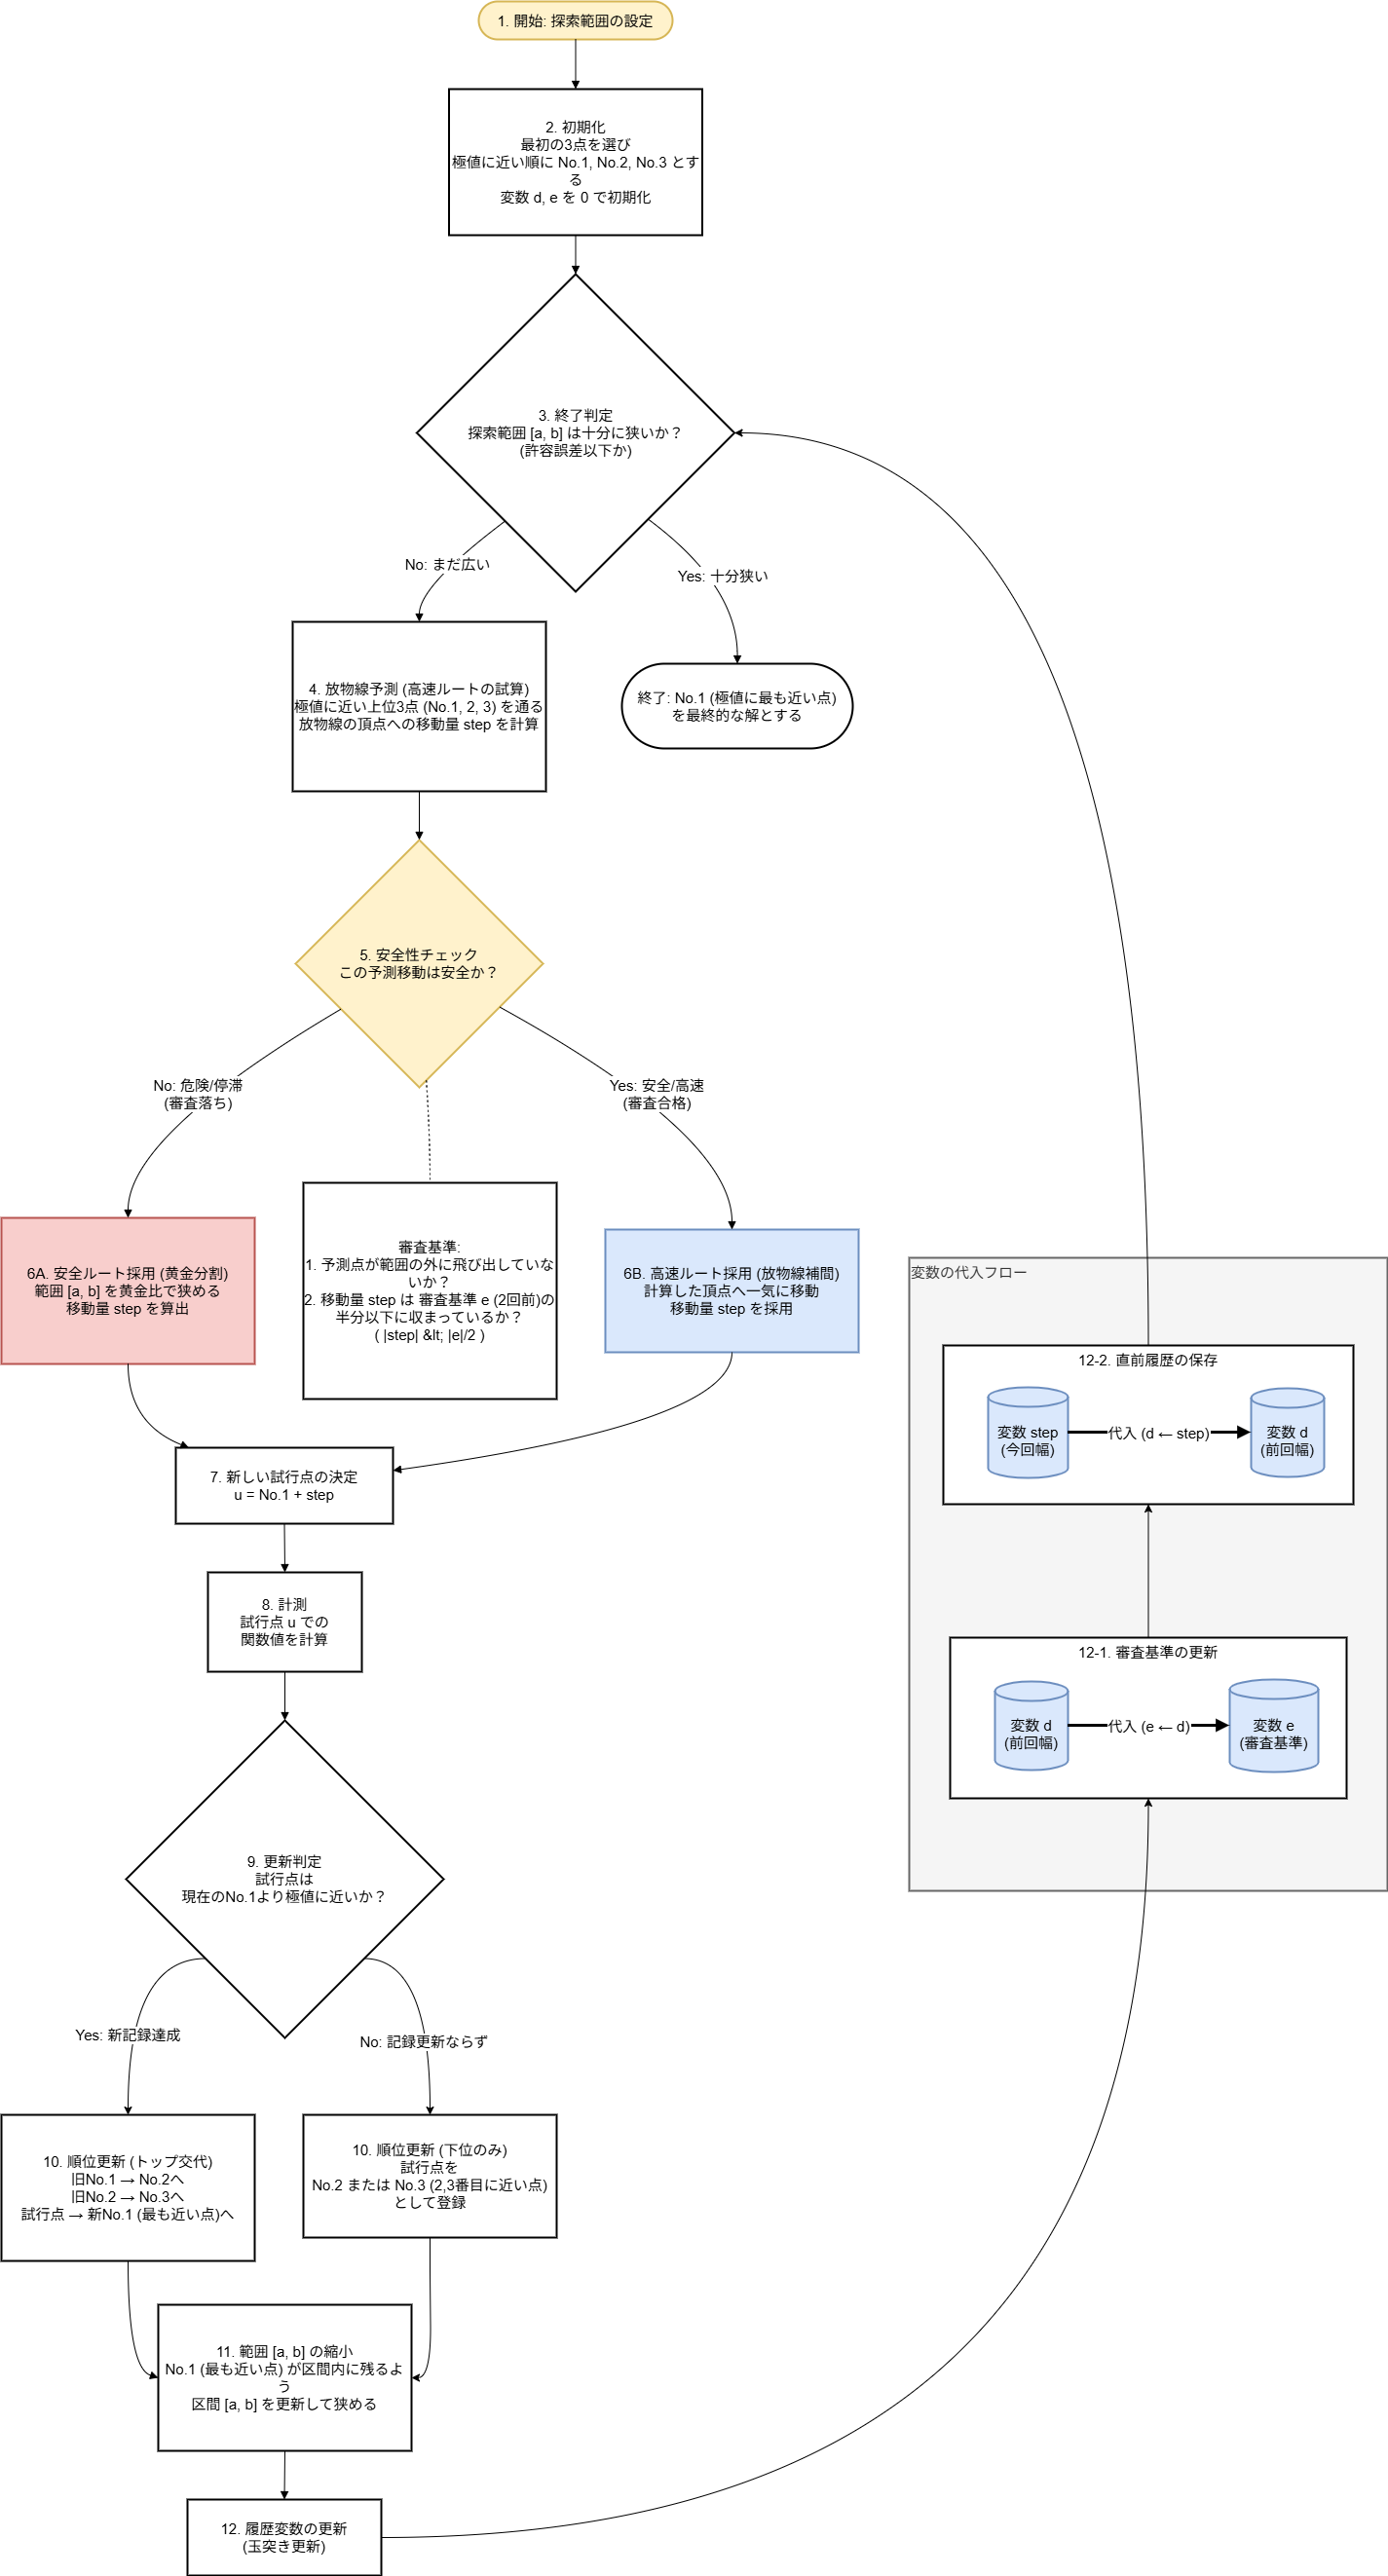
\includegraphics[width=0.7\linewidth]{material/brent/brent-architecture.png}
    \caption{Brent法のアルゴリズム構成}
  \end{figure}

\subsection{収束の様子}
  \begin{figure}[H]
    \begin{minipage}[b]{0.48\linewidth}
      \centering
      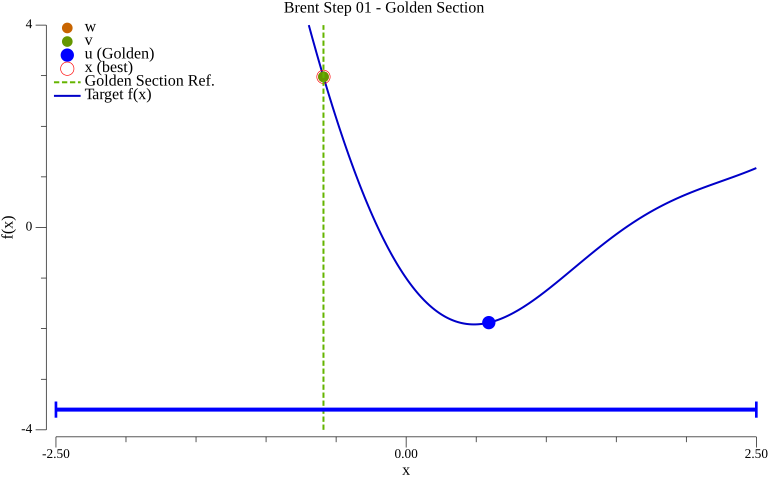
\includegraphics[width=1.0\linewidth]{material/brent/brent-step-01.png}
      \caption{Brent法-01回目}
    \end{minipage}
    \hfill
    \begin{minipage}[b]{0.48\linewidth}
      \centering
      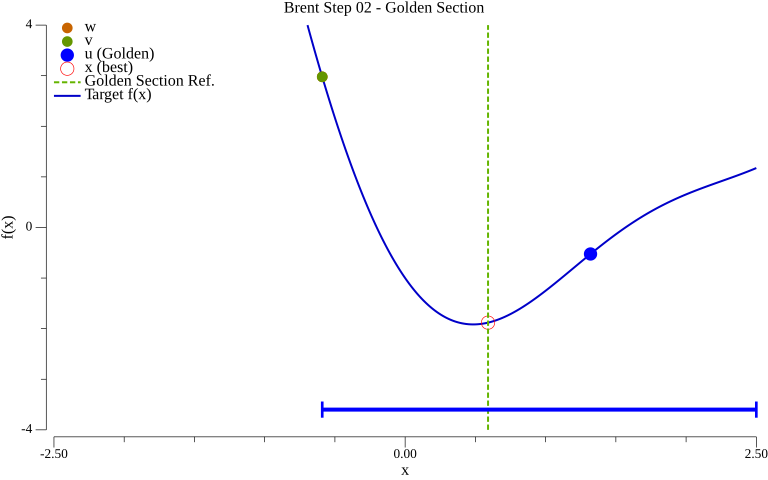
\includegraphics[width=1.0\linewidth]{material/brent/brent-step-02.png}
      \caption{Brent法-02回目}
    \end{minipage}
  \end{figure}
  \begin{figure}[H]
    \begin{minipage}[b]{0.48\linewidth}
      \centering
      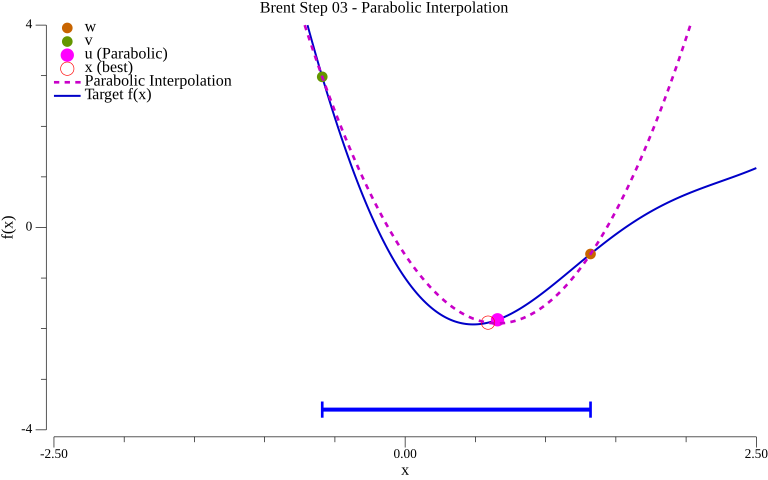
\includegraphics[width=1.0\linewidth]{material/brent/brent-step-03.png}
      \caption{Brent法-03回目}
    \end{minipage}
    \hfill
    \begin{minipage}[b]{0.48\linewidth}
      \centering
      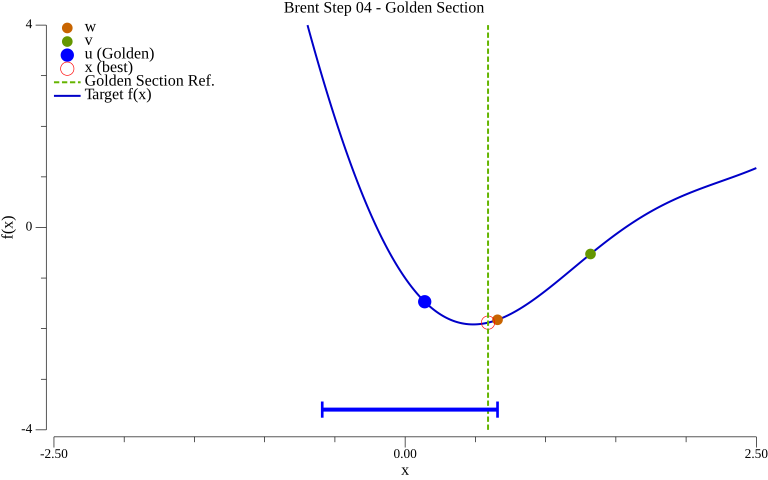
\includegraphics[width=1.0\linewidth]{material/brent/brent-step-04.png}
      \caption{Brent法-04回目}
    \end{minipage}
  \end{figure}
  \begin{figure}[H]
    \begin{minipage}[b]{0.48\linewidth}
      \centering
      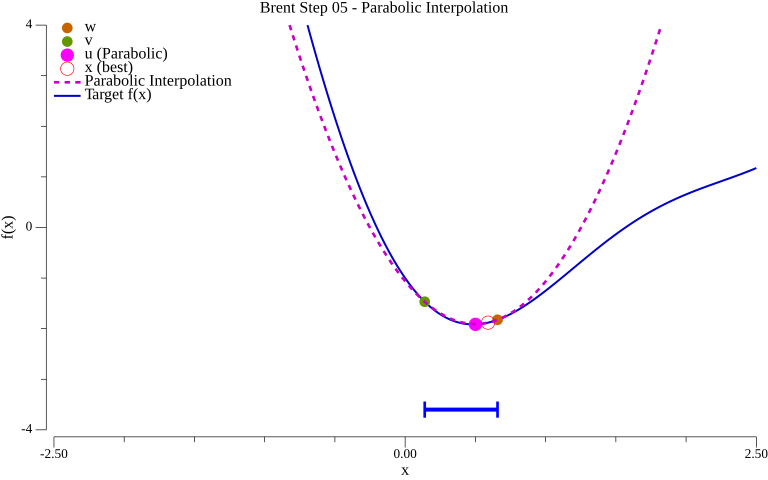
\includegraphics[width=1.0\linewidth]{material/brent/brent-step-05.png}
      \caption{Brent法-05回目}
    \end{minipage}
    \hfill
    \begin{minipage}[b]{0.48\linewidth}
      \centering
      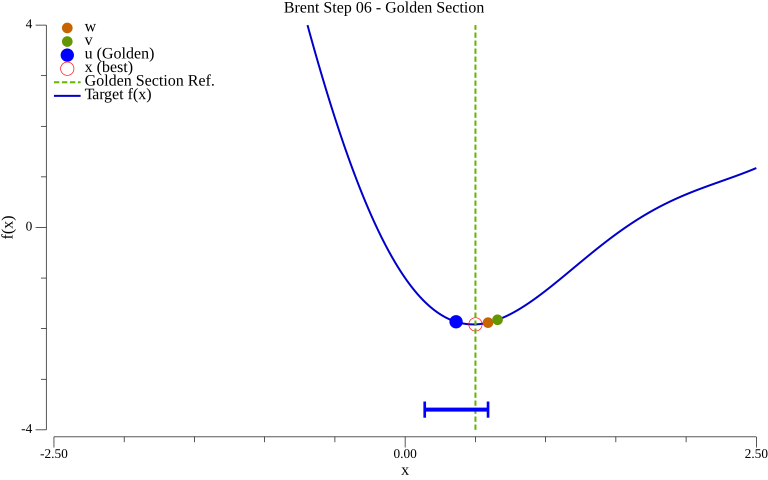
\includegraphics[width=1.0\linewidth]{material/brent/brent-step-06.png}
      \caption{Brent法-06回目}
    \end{minipage}
  \end{figure}
  \begin{figure}[H]
    \begin{minipage}[b]{0.48\linewidth}
      \centering
      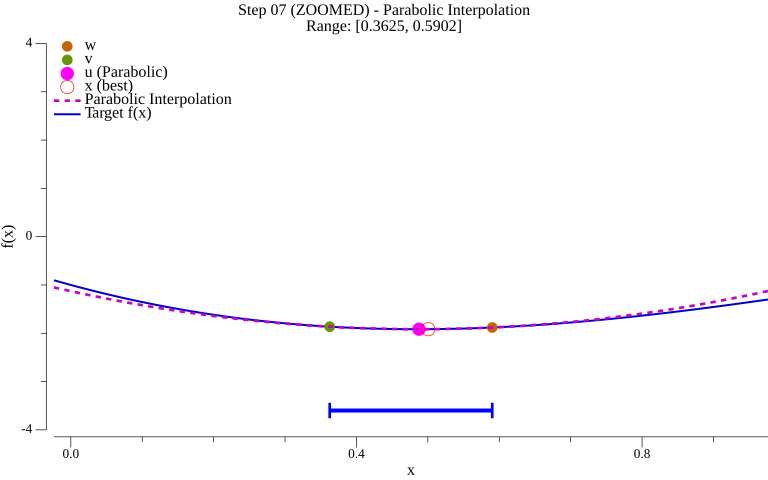
\includegraphics[width=1.0\linewidth]{material/brent/brent-step-07.png}
      \caption{Brent法-07回目}
    \end{minipage}
    \hfill
    \begin{minipage}[b]{0.48\linewidth}
      \centering
      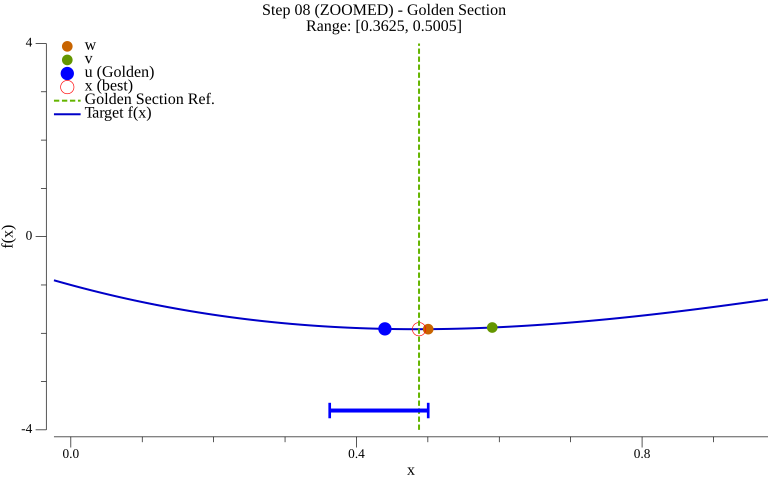
\includegraphics[width=1.0\linewidth]{material/brent/brent-step-08.png}
      \caption{Brent法-08回目}
    \end{minipage}
  \end{figure}
  \begin{figure}[H]
    \begin{minipage}[b]{0.48\linewidth}
      \centering
      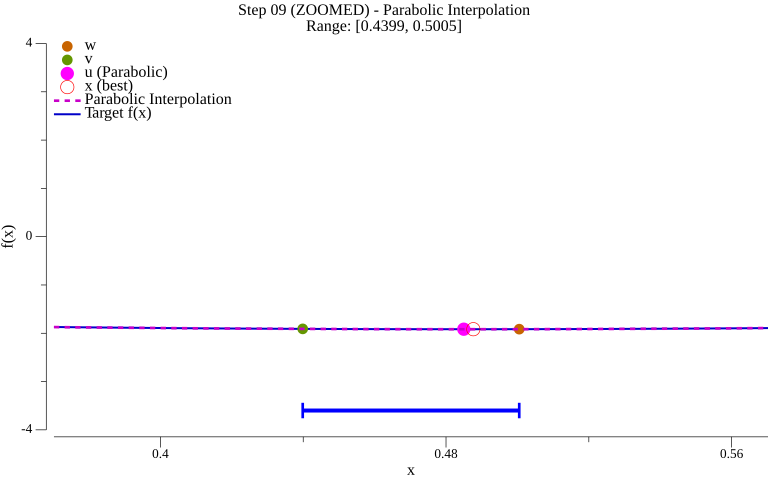
\includegraphics[width=1.0\linewidth]{material/brent/brent-step-09.png}
      \caption{Brent法-09回目}
    \end{minipage}
    \hfill
    \begin{minipage}[b]{0.48\linewidth}
      \centering
      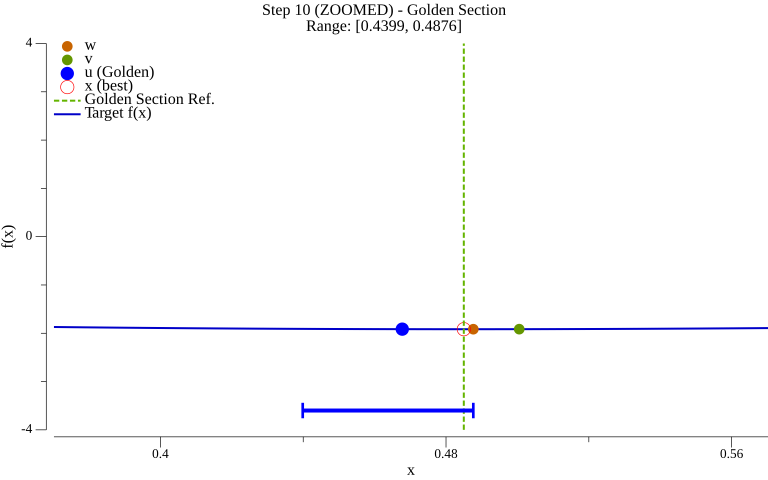
\includegraphics[width=1.0\linewidth]{material/brent/brent-step-10.png}
      \caption{Brent法-10回目}
    \end{minipage}
  \end{figure}
  \begin{figure}[H]
    \begin{minipage}[b]{0.48\linewidth}
      \centering
      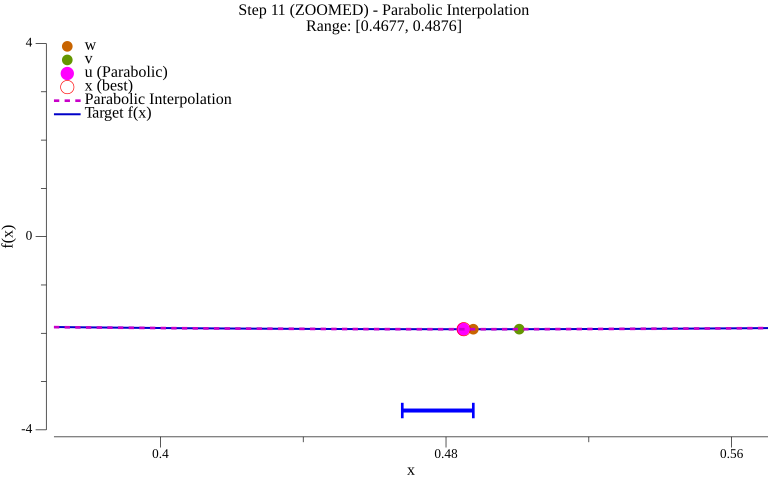
\includegraphics[width=1.0\linewidth]{material/brent/brent-step-11.png}
      \caption{Brent法-11回目}
    \end{minipage}
    \hfill
    \begin{minipage}[b]{0.48\linewidth}
      \centering
      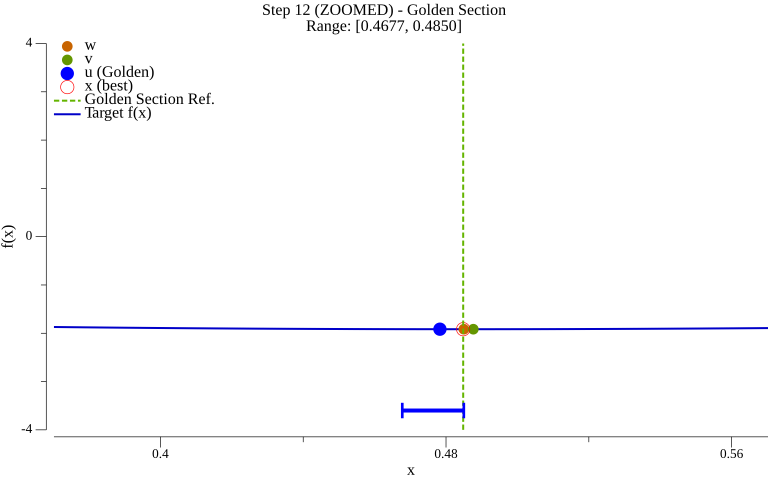
\includegraphics[width=1.0\linewidth]{material/brent/brent-step-12.png}
      \caption{Brent法-12回目}
    \end{minipage}
  \end{figure}
  \begin{figure}[H]
    \begin{minipage}[b]{0.48\linewidth}
      \centering
      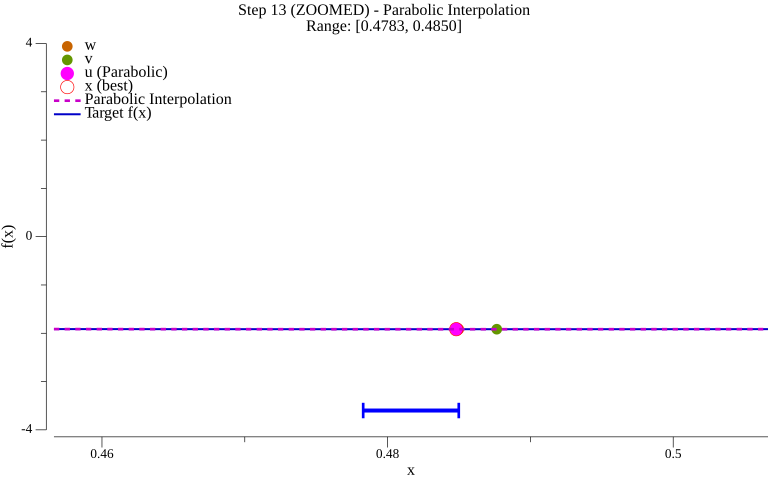
\includegraphics[width=1.0\linewidth]{material/brent/brent-step-13.png}
      \caption{Brent法-13回目}
    \end{minipage}
    \hfill
    \begin{minipage}[b]{0.48\linewidth}
      \centering
      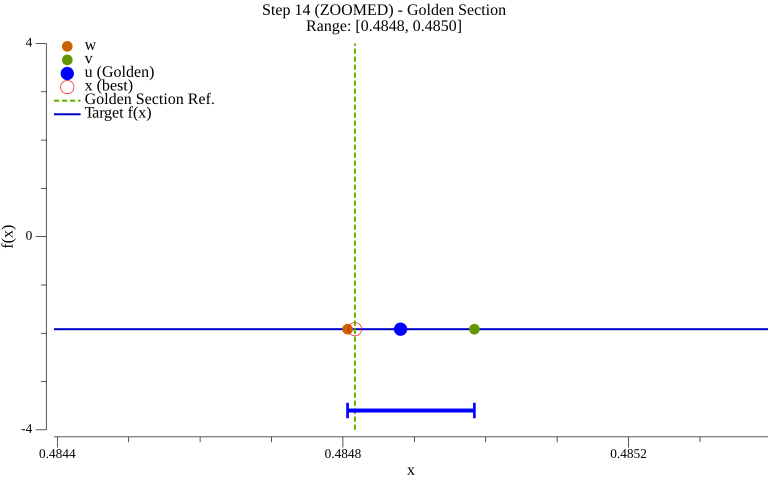
\includegraphics[width=1.0\linewidth]{material/brent/brent-step-14.png}
      \caption{Brent法-14回目}
    \end{minipage}
  \end{figure}
  \begin{figure}[H]
    \begin{minipage}[b]{0.48\linewidth}
      \centering
      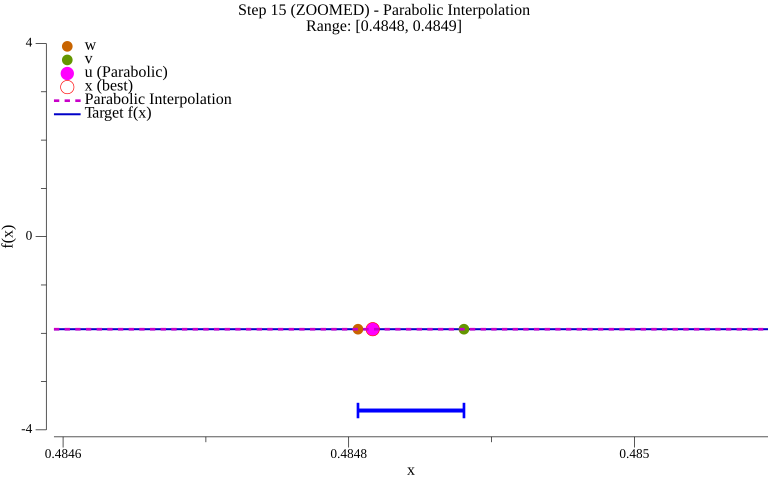
\includegraphics[width=1.0\linewidth]{material/brent/brent-step-15.png}
      \caption{Brent法-15回目}
    \end{minipage}
    \hfill
    \begin{minipage}[b]{0.48\linewidth}
      \centering
      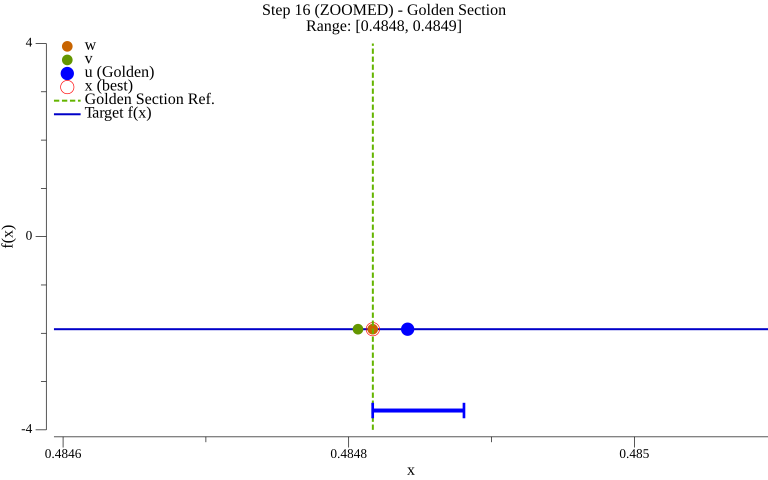
\includegraphics[width=1.0\linewidth]{material/brent/brent-step-16.png}
      \caption{Brent法-16回目}
    \end{minipage}
  \end{figure}
  \begin{figure}[H]
    \begin{minipage}[b]{0.48\linewidth}
      \centering
      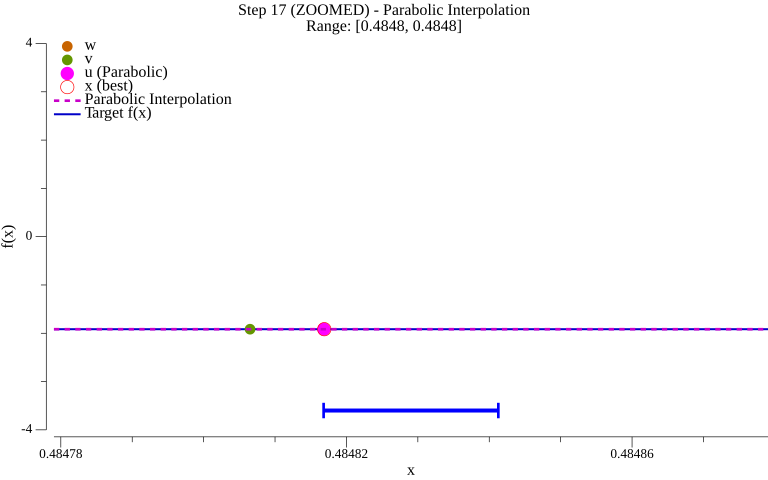
\includegraphics[width=1.0\linewidth]{material/brent/brent-step-17.png}
      \caption{Brent法-17回目}
    \end{minipage}
    \hfill
    \begin{minipage}[b]{0.48\linewidth}
      \centering
      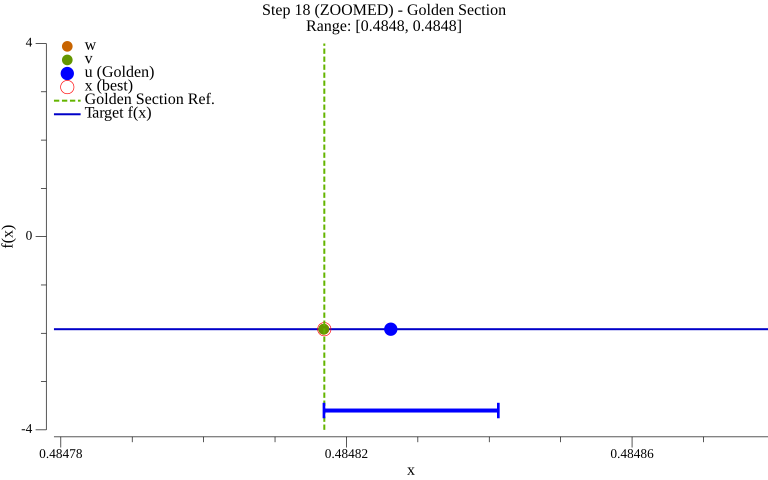
\includegraphics[width=1.0\linewidth]{material/brent/brent-step-18.png}
      \caption{Brent法-18回目}
    \end{minipage}
  \end{figure}
  \begin{figure}[H]
    \begin{minipage}[b]{0.48\linewidth}
      \centering
      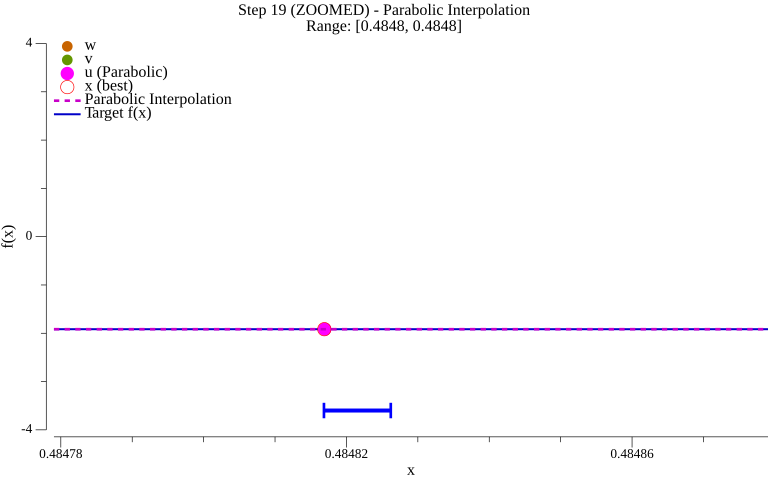
\includegraphics[width=1.0\linewidth]{material/brent/brent-step-19.png}
      \caption{Brent法-19回目}
    \end{minipage}
  \end{figure}
  \begin{figure}[H]
    \centering
    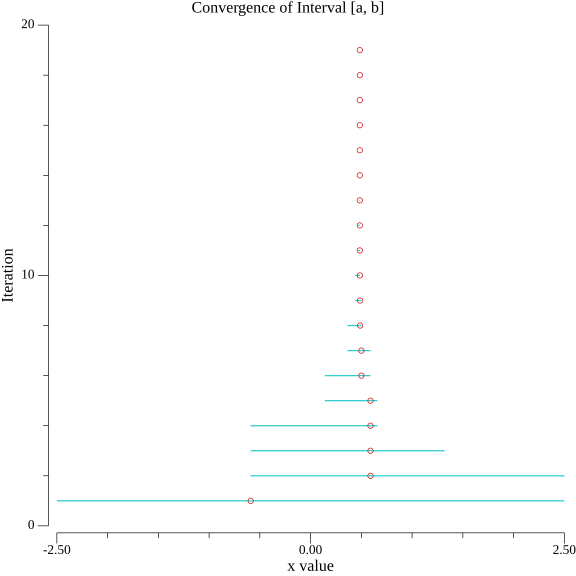
\includegraphics[width=0.7\linewidth]{material/brent/brent-interval.png}
    \caption{Brent法: 探索区間の収束推移}
  \end{figure}


\newpage  %% 改ページ ==================================================

% 第5章 Brent法を用いたRemesアルゴリズム
\section{Brent法を用いたRemesアルゴリズムの実装と評価}
\label{sec:brent_remes_impl}

前章までに述べた通り，Remesアルゴリズムの収束精度は，その内部で行われる「極値探索（Step 2）」の精度に完全に依存している．
第3章の予備実験では，単純なグリッド極値点探索を用いた場合，グリッド間隔に依存した離散化誤差が避けられず，交替定理を数値的に満たす解（最良近似多項式）に到達できないことが確認された．

本章では，この課題を解決するために，第4章で解説したBrent法をRemesアルゴリズムの極値探索エンジンとして組み込んだ手法を提案する．
本手法は，微分を用いない最適化手法でありながら，放物線補間と黄金分割探索を組み合わせることで，機械イプシロンの精度限界まで高速に極値を特定することを可能にする．

\subsection{実装アルゴリズムの詳細}
  \label{subsec:impl_algorithm}
本研究で実装した改良型Remesアルゴリズムは，以下の3段階のプロセスを経て参照点を更新する．
この手順は，数値的な安定性と交替定理の条件（符号の交互性）を維持するために慎重に設計されている．

\subsubsection{Phase 1: 誤差関数の根の探索と区間分割}
多項式近似において，誤差関数 $e(x) = f(x) - P(x)$ の極値は，必ずその「根（$e(x)=0$ となる点）」の間に存在する．
そこで，まずは大まかなグリッド極値点探索を用いて $e(x)$ の符号が変化する区間を見つけ，二分法（Bisection Method）を用いて根の位置 $z_0, z_1, \dots, z_{n}$ を数値的に推定する．

これにより，定義域 $[a, b]$ は，誤差関数の符号が一定であるような $n+2$ 個の部分区間 $I_j$ に分割される．
\[
I_0 = [a, z_0], \quad I_1 = [z_0, z_1], \quad \dots, \quad I_{n+1} = [z_n, b].
\]
この操作により，各区間内には必ず一つ以上の極値が存在し，かつ隣り合う区間では極値の符号が逆になることが保証される．

\subsubsection{Phase 2: Brent法による極値の高精度な特定}
分割された各区間 $I_j$ において，Brent法を用いて誤差の絶対値 $|e(x)|$ が最大となる点 $\xi_j$ を探索する．
ここで，目的関数を $g(x) = -|e(x)|$ と設定し，これを最小化する問題を解く．

Brent法の収束判定条件（許容誤差 tol）には，倍精度浮動小数点数の機械イプシロンに近い $10^{-15}$ を設定した．
これにより，グリッド極値点探索のような離散的な点ではなく，連続的な実数空間上での真の極値を，計算機が表現できる限界の精度でピンポイントに特定することが期待される．

\subsubsection{Phase 3: 参照点の更新}
各区間で得られた極値候補 $\xi_0, \dots, \xi_{n+1}$ を新しい参照点として採用する．
このとき，もし候補点が区間の境界（根や定義域の端点）に極端に近い場合は，数値的不安定性を避けるための微小な補正を行うが，Brent法が正常に収束していれば，通常これらの点は交替定理を満たす理想的な配置となる．

\subsection{数値実験の設定}
  \label{subsec:numerical_experiment}
提案手法の性能を検証するため，多項式近似において「悪条件」として知られるルンゲ関数を対象に，高次多項式による近似実験を行った．

\begin{itemize}
    \item \textbf{近似対象関数}: $f(x) = \frac{1}{1+25x^2}.$
    \item \textbf{定義域}: $[-1, 1].$
    \item \textbf{近似多項式の次数}: $n=15.$
    \item \textbf{比較対象}: 第3章で実装したグリッド極値点探索法（分割数 $N=2000$）.
    \item \textbf{評価指標}:
    \begin{enumerate}
        \item \textbf{収束速度}: 何回の反復で収束判定（Error $< 10^{-14}$）に至ったか．
        \item \textbf{到達精度}: 最終的な誤差のばらつき（Spread）がどの程度まで小さくなったか．
        \item \textbf{残留誤差}: 収束後の多項式に対し，さらに高精度な再評価を行った際に検出される誤差．
    \end{enumerate}
\end{itemize}

\subsection{実験結果と解析}

\subsubsection{収束過程の推移}
数値実験により得られた収束ログを表\ref{tab:remes-brent-log}に，その推移グラフを図\ref{fig:remes-brent-convergence}に示す．

% =========================================================
% Goプログラム (remes_brent.go) が生成した結果を読み込む
% =========================================================
%% 5章用 (Brent)

以下の図表は，Brent法による極値探索を用いて，関数 $f(x) = \frac{1}{1+25x^2}$ ($n=15$) を近似した際の収束過程を示したものである．

表\ref{tab:remes-brent-log}は，各反復で算出された参照均等誤差 $|E|$ と，Brent法で高精度に求められた実際の最大誤差，およびその差の推移である．
グリッド極値点探索と比較して，より高精度な収束（$10^{-15}$ オーダー）が達成されている．

図\ref{fig:remes-brent-convergence}は，反復に伴う誤差の収束過程を可視化したものである．
Brent法により，機械イプシロン精度に近い等振動性が実現されていることが確認できる．


\begin{figure}[H]
 \centering
 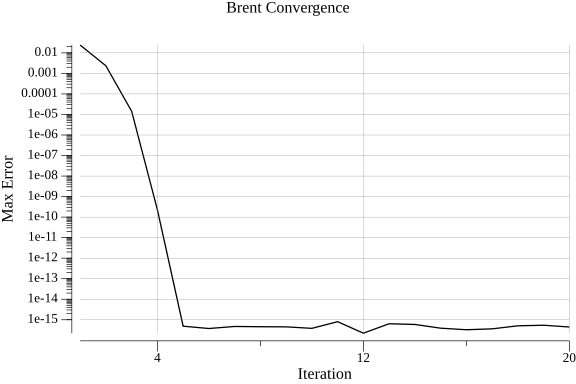
\includegraphics[width=0.6\linewidth]{material/remes/outputs/brent/convergence_brent.png}
 \caption{Brent法による最大誤差の収束履歴}
 \label{fig:remes-brent-convergence}
\end{figure}

\begin{figure}[H]
 \centering
 \begin{minipage}[b]{0.48\textwidth}
  \centering
  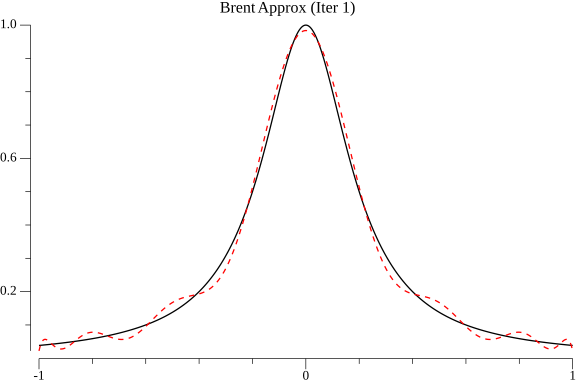
\includegraphics[width=1.0\linewidth]{material/remes/outputs/brent/func_remes_brent_iter01.png}
  \caption{Iter 1}
 \end{minipage}
 \hfill
 \begin{minipage}[b]{0.48\textwidth}
  \centering
  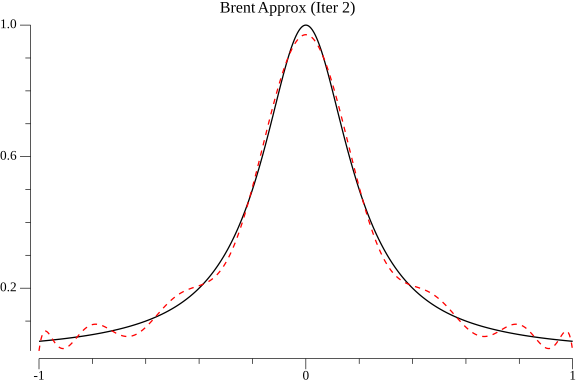
\includegraphics[width=1.0\linewidth]{material/remes/outputs/brent/func_remes_brent_iter02.png}
  \caption{Iter 2}
 \end{minipage}

 \begin{minipage}[b]{0.48\textwidth}
  \centering
  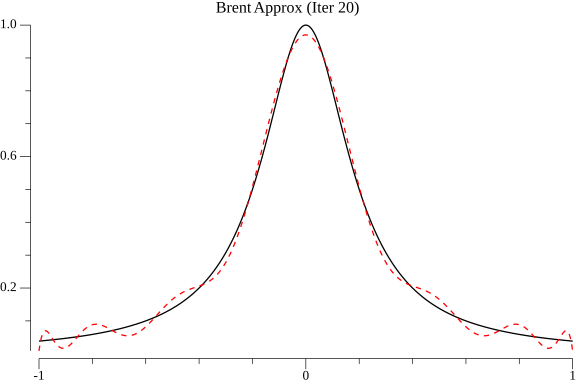
\includegraphics[width=1.0\linewidth]{material/remes/outputs/brent/func_remes_brent_iter20.png}
  \caption{Iter 20}
 \end{minipage}

 \caption{Brent法: 近似多項式の推移}
 \label{fig:remes-brent-approx}
\end{figure}
\begin{figure}[H]
 \centering
 \begin{minipage}[b]{0.48\textwidth}
  \centering
  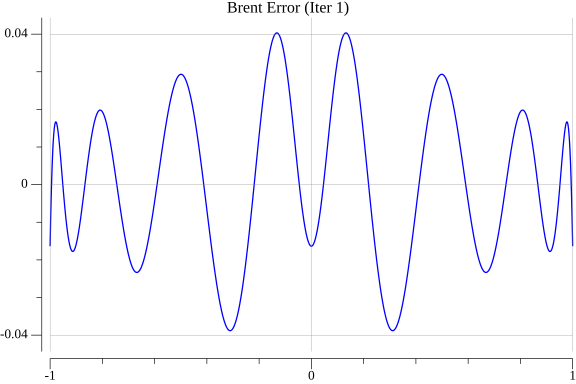
\includegraphics[width=1.0\linewidth]{material/remes/outputs/brent/error_remes_brent_iter01.png}
  \caption{Iter 1}
 \end{minipage}
 \hfill
 \begin{minipage}[b]{0.48\textwidth}
  \centering
  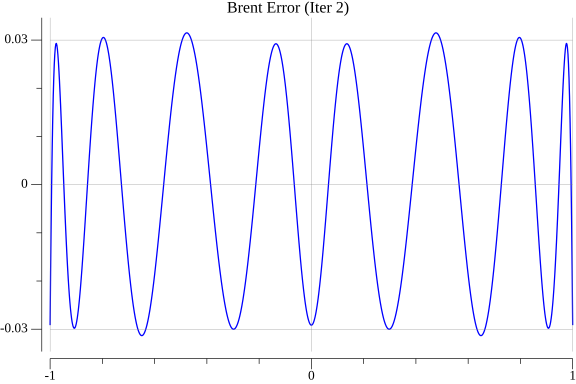
\includegraphics[width=1.0\linewidth]{material/remes/outputs/brent/error_remes_brent_iter02.png}
  \caption{Iter 2}
 \end{minipage}

 \begin{minipage}[b]{0.48\textwidth}
  \centering
  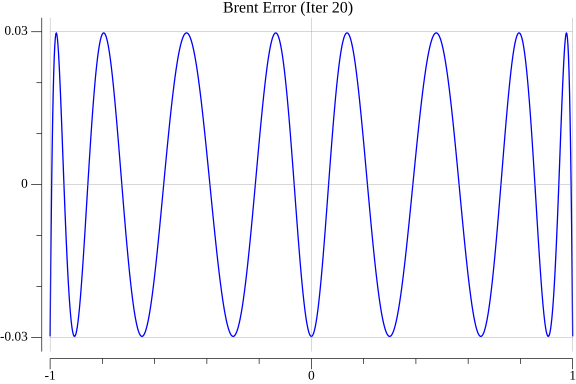
\includegraphics[width=1.0\linewidth]{material/remes/outputs/brent/error_remes_brent_iter20.png}
  \caption{Iter 20}
 \end{minipage}

 \caption{Brent法: 誤差関数の推移}
 \label{fig:remes-brent-error}
\end{figure}

\begin{table}[H]
 \centering
 \caption{Brent法の収束ログ}
 \label{tab:remes-brent-log}
 \begin{tabular}{crrrr}
 \toprule
 Iter & $|E|$ & Coeff Norm & Node Move & Error Change \\
 \midrule
 1 & $1.63552e-02$ & $0.00000e+00$ & $0.00000e+00$ & $0.00000e+00$ \\
 2 & $2.91586e-02$ & $1.38180e-02$ & $4.97122e-02$ & $1.28034e-02$ \\
 3 & $2.97711e-02$ & $1.27592e-03$ & $3.72393e-03$ & $6.12455e-04$ \\
 4 & $2.97767e-02$ & $6.60148e-06$ & $1.24099e-05$ & $5.62755e-06$ \\
 5 & $2.97767e-02$ & $1.05586e-10$ & $5.25736e-09$ & $9.91564e-11$ \\
 6 & $2.97767e-02$ & $1.62634e-16$ & $5.64624e-09$ & $6.24500e-17$ \\
 7 & $2.97767e-02$ & $2.07658e-16$ & $4.94056e-09$ & $6.93889e-18$ \\
 8 & $2.97767e-02$ & $2.55847e-16$ & $4.96228e-09$ & $2.42861e-17$ \\
 9 & $2.97767e-02$ & $1.62274e-16$ & $3.21817e-09$ & $3.46945e-18$ \\
 10 & $2.97767e-02$ & $2.38584e-16$ & $3.65966e-09$ & $6.93889e-18$ \\
 11 & $2.97767e-02$ & $2.28951e-16$ & $4.44502e-09$ & $1.73472e-17$ \\
 12 & $2.97767e-02$ & $2.19203e-16$ & $3.89086e-09$ & $0.00000e+00$ \\
 13 & $2.97767e-02$ & $1.66362e-16$ & $4.61242e-09$ & $6.93889e-18$ \\
 14 & $2.97767e-02$ & $2.27033e-16$ & $4.29365e-09$ & $2.42861e-17$ \\
 15 & $2.97767e-02$ & $2.48827e-16$ & $4.68158e-09$ & $2.77556e-17$ \\
 16 & $2.97767e-02$ & $1.87220e-16$ & $5.47251e-09$ & $5.89806e-17$ \\
 17 & $2.97767e-02$ & $1.19187e-16$ & $6.30429e-09$ & $7.97973e-17$ \\
 18 & $2.97767e-02$ & $1.93991e-16$ & $3.62033e-09$ & $3.12250e-17$ \\
 19 & $2.97767e-02$ & $2.77619e-16$ & $4.55541e-09$ & $7.63278e-17$ \\
 20 & $2.97767e-02$ & $1.85424e-16$ & $5.41280e-09$ & $7.63278e-17$ \\
 \bottomrule
 \end{tabular}
\end{table}

\begin{table}[H]
 \centering
 \caption{Brent法利用時の誤差の再評価}
 \label{tab:remes-brent-final-check}
 \begin{tabular}{crrr}
 \toprule
 No. & 収束時誤差 & 再評価誤差 & 差分 \\
 \midrule
 1 & $2.97766890e-02$ & $2.97766890e-02$ & $9.60343e-15$ \\
 2 & $2.97766890e-02$ & $2.97766890e-02$ & $0.00000e+00$ \\
 3 & $2.97766890e-02$ & $2.97766890e-02$ & $-1.38778e-17$ \\
 4 & $2.97766890e-02$ & $2.97766890e-02$ & $6.93889e-18$ \\
 5 & $2.97766890e-02$ & $2.97766890e-02$ & $0.00000e+00$ \\
 6 & $2.97766890e-02$ & $2.97766890e-02$ & $-2.77556e-17$ \\
 7 & $2.97766890e-02$ & $2.97766890e-02$ & $0.00000e+00$ \\
 8 & $2.97766890e-02$ & $2.97766890e-02$ & $0.00000e+00$ \\
 9 & $2.97766890e-02$ & $2.97766890e-02$ & $0.00000e+00$ \\
 10 & $2.97766890e-02$ & $2.97766890e-02$ & $0.00000e+00$ \\
 11 & $2.97766890e-02$ & $2.97766890e-02$ & $0.00000e+00$ \\
 12 & $2.97766890e-02$ & $2.97766890e-02$ & $-2.77556e-17$ \\
 13 & $2.97766890e-02$ & $2.97766890e-02$ & $-6.93889e-18$ \\
 14 & $2.97766890e-02$ & $2.97766890e-02$ & $-1.38778e-17$ \\
 15 & $2.97766890e-02$ & $2.97766890e-02$ & $6.93889e-18$ \\
 16 & $2.97766890e-02$ & $2.97766890e-02$ & $0.00000e+00$ \\
 17 & $2.97766890e-02$ & $2.97766890e-02$ & $8.93036e-15$ \\
 \bottomrule
 \end{tabular}
\vspace{1mm}

\small \textbf{注：}
\small 上表は，区間 $[-1.0,1.0]$ を探索するRemesアルゴリズムによって導かれた誤差関数に対する表である．

\small 収束時誤差とはBrent法をもちいることで極値点探索を行ったRemesアルゴリズムで導出された誤差関数の各極値点で観測された誤差である．

\small 再評価誤差とはBrent法という極値点探索アルゴリズムにより観測された誤差の絶対値である．

\[
 \text{観測された最大誤差} \; \|E\|_{\max}^{\text{strict}}(f) = \max_{x \in [-1.0,1.0]} |f(x) - p^*(x)| \approx 2.97766890e-02 .
 \]
\end{table}


表\ref{tab:remes-brent-log}を見ると，反復の初期段階（Iter 1〜5）では誤差のばらつき（Spread）が比較的大きいが，Iter 6以降で急激に減少し，Iter 10付近では $10^{-16}$ のオーダーに達していることがわかる．
これは，第3章で確認されたRemesアルゴリズムの「2次収束」の特性が，Brent法による高精度な極値探索によって最大限に引き出された結果であると言える．

図\ref{fig:remes-brent-convergence}は，その過程における収束の様子を可視化したものである．
初期のイテレーションでは誤差関数の波形が大きく乱れているが，最終的には振幅が一定な「等振動（Equioscillation）」の状態へと収束している．

\subsubsection{近似度の検証：グリッド極値点探索との決定的差異}
表\ref{tab:remes-brent-final-check}（末尾）は，収束した多項式に対して，再度Brent法を用いて全極値を精査し，その誤差絶対値を比較したものである．

この表における「差分」に注目すると，すべての極値においてその値は $10^{-15}$ 〜 $10^{-17}$ のオーダーに収まっている．
これは，第3章のグリッド極値点探索で残っていた $10^{-9}$ 程度の誤差と比較して，$10^{7}$ 倍（1000万倍）以上の精度向上を達成したことを意味する．
すなわち，本実装によって得られた多項式は，倍精度演算の枠内において「これ以上改善しようがない」レベルの最良近似多項式であると断言できる．


% 第6章 考察
\section{考察}
\label{sec:discussion}

本章では，第3章で実装したグリッド極値点探索法と，第5章で提案したBrent法を用いたRemesアルゴリズムの性能を比較し，その差異が生じた数理的な要因について考察する．

\subsection{極値探索における残留誤差の定量評価}
  \label{subsec:residual_error}
まず，両手法によって得られた「最良近似多項式」が，交替定理を満たしているかを検証する．
以下の図表は，収束後の多項式に対し，さらに高精度な探索を行って検出された「残留誤差（見逃された誤差）」等の比較結果である．

% =========================================================
% Goプログラムが生成した比較結果（図表）をここで読み込む
% このファイルの中に 表5, 表6, 図52 が定義されています
% =========================================================
%% 6章用 (Comparison)

以下の図表は，グリッド極値点探索法とBrent法の性能を比較したものである（対象関数: $f(x) = \frac{1}{1+25x^2}$，次数: $n=15$）．

表\ref{tab:remes-comparison-summary}は，両手法の収束性能，計算時間，最終精度を比較した総合評価である．
Brent法は計算時間がやや増加するものの，極値探索精度の向上により，より高精度な最良近似多項式が得られることが示されている．

図\ref{fig:remes-comparison-deviation}は，各極値点における理論値からの偏差を可視化したものである．
グリッド極値点探索では離散化誤差により微小なズレが残るのに対し，Brent法では機械イプシロンレベルの精度が達成されている．

\begin{figure}[H]
 \centering
 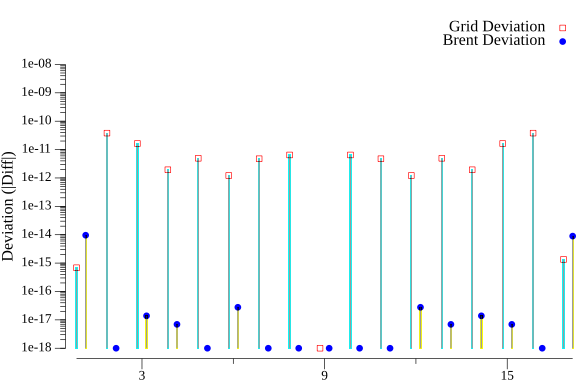
\includegraphics[width=0.8\linewidth]{material/remes/outputs/comparison/deviation_comparison.png}
 \caption{極値点ごとの理論値からの偏差 ($|\text{Calc} - \text{True}|$)}
 \label{fig:remes-comparison-deviation}
\end{figure}

\begin{table}[H]
 \centering
 \caption{グリッド法とBrent法の性能比較概要 ($n=15$)}
 \label{tab:remes-comparison-summary}
 \begin{tabular}{lcccc}
 \toprule
 手法 & 反復回数 & 収束判定値 & 高精度な最大誤差 $\|E\|$ & 計算時間 \\
 \midrule
 Grid Search & 6 & $6.10623e-16$ & $2.97811e-02$ & 268.04403ms \\
 Brent Method & 20 & $4.44089e-16$ & $2.97767e-02$ & 796.27914ms \\
 \bottomrule
 \end{tabular}
\vspace{1mm}

\footnotesize\textbf{高精度な最大誤差について：}
区間 $[-1.0,1.0]$ を50,000個の格子点で均等分割し，誤差関数 $|E(x)|$ の局所極大値を検出した後，
各極大値の近傍に対してBrent法を適用して算出した値である．
\end{table}

\begin{table}[H]
 \centering
 \caption{各極値点における真の誤差との偏差比較（等振幅性の崩れ）}
 \label{tab:remes-comparison-detail}
 \begin{tabular}{crrr}
 \toprule
 No. & Grid偏差 ($|\Delta E|$) & Brent偏差 ($|\Delta E|$) & 精度比 (Grid/Brent) \\
 \midrule
 1 & $6.86950e-16$ & $9.60343e-15$ & $0.1$ \\
 2 & $3.80066e-11$ & $0.00000e+00$ & $0.0$ \\
 3 & $1.63316e-11$ & $1.38778e-17$ & $1176819.0$ \\
 4 & $1.94925e-12$ & $6.93889e-18$ & $280916.0$ \\
 5 & $4.93021e-12$ & $0.00000e+00$ & $0.0$ \\
 6 & $1.21936e-12$ & $2.77556e-17$ & $43932.0$ \\
 7 & $4.76352e-12$ & $0.00000e+00$ & $0.0$ \\
 8 & $6.46216e-12$ & $0.00000e+00$ & $0.0$ \\
 9 & $0.00000e+00$ & $0.00000e+00$ & $0.0$ \\
 10 & $6.46216e-12$ & $0.00000e+00$ & $0.0$ \\
 11 & $4.76358e-12$ & $0.00000e+00$ & $0.0$ \\
 12 & $1.21927e-12$ & $2.77556e-17$ & $43929.0$ \\
 13 & $4.93020e-12$ & $6.93889e-18$ & $710517.0$ \\
 14 & $1.94927e-12$ & $1.38778e-17$ & $140459.5$ \\
 15 & $1.63316e-11$ & $6.93889e-18$ & $2353638.0$ \\
 16 & $3.80066e-11$ & $0.00000e+00$ & $0.0$ \\
 17 & $1.34615e-15$ & $8.93036e-15$ & $0.2$ \\
 \bottomrule
 \end{tabular}
\end{table}

\noindent\textbf{考察:}
表\ref{tab:remes-comparison-summary}において，全区間を対象とした高精度な再評価を行った結果，
Grid法の最大誤差 $\|E\|$ は $2.978113e-02$ となり，Brent法の $2.977669e-02$ よりも大きな値を示した．
これは，Grid法が離散的な探索により真の最大誤差（ピーク）を取りこぼして収束していたことを示唆しており，
Brent法を用いることで，より最大誤差が小さく，最良近似多項式に近い結果が得られたことを裏付けている．
また，表\ref{tab:remes-comparison-detail}に示すように，各極値点における等振幅性の偏差はBrent法の方が平均して約 7905 倍小さく，
数学的性質の観点からもBrent法がより高精度な近似解を得られていることが確認できる．


表\ref{tab:remes-comparison-detail}（各極値点における真の誤差との偏差比較）が示す通り，グリッド極値点探索法では収束判定後も各極値点において平均 $10^{-11}$ 程度の誤差が残留している．これは，グリッドの刻み幅 $\Delta x$ に依存する離散化誤差が避けられないためである．

一方，Brent法を用いた場合，残留誤差は $10^{-15} \sim 10^{-17}$ のオーダーであり，これは倍精度浮動小数点数における機械イプシロン（約 $2.22 \times 10^{-16}$）と同等である．
この結果から，Brent法は計算機が表現可能な限界の精度で極値を特定できていると言える．

\subsection{逆放物線補間による高精度化のメカニズム}

なぜBrent法は，グリッド極値点探索と変わらない計算時間（表\ref{tab:remes-comparison-summary}参照）でこれほどの高精度を実現できたのか．その理由は，Brent法のアルゴリズムの中核にある「逆放物線補間（Inverse Parabolic Interpolation）」にある．

Remesアルゴリズムが収束に近づくにつれて，誤差関数 $e(x)$ の極値付近の挙動は，滑らかな放物線に近似できるようになる．
第4章で述べたように，Brent法は3点 $(x, w, v)$ を通る放物線の頂点を推定して次の探索点を選ぶ\cite{brent-original}．
グリッド極値点探索が「しらみつぶし」に点を探すのに対し，Brent法は関数の形状（曲率）を利用して，極値の場所を「予測」して飛び込むことができる．

本実験の結果は，Remesアルゴリズムにおける誤差関数の極値探索において，この放物線近似が極めて有効に機能したことを示唆している．

\subsection{Remesアルゴリズムの2次収束性の実現}

\ref{subsec:newton_equivalence}の理論的背景で述べたように，Remesアルゴリズム（全点同時入れ替え法）は，参照点が真の極値に近い場合，ニュートン法と同様に2次収束する特性を持つ\cite{seminar-note}．

しかし，この理論的収束速度を実現するためには，各ステップにおける極値探索が十分な精度で行われていることが前提条件となる．
$2000$グリッド極値点探索の場合，極値の特定精度が $10^{-11}$ 程度で頭打ちになるため，Remesアルゴリズム自体の収束もそこで阻害され，本来の2次収束の性能を活かしきれない．

対して，Brent法を導入した本手法では，極値を機械精度まで正確に特定できるため，Remesアルゴリズムの理論通りの2次収束が維持され，結果として $10^{-16}$ オーダーの高精度な最良近似多項式を導出することに成功したと考えられる．


% 第7章 結論
\section{結論}
\label{sec:conclusion}

本研究では，最良近似多項式の導出における「極値探索」の精度に着目し，Brent法を導入した高精度なRemesアルゴリズムの実装を行った．
数値実験の結果，ルンゲ関数のような悪条件の問題に対しても，提案手法はグリッド極値点探索法と比較して圧倒的に高い精度で交替定理を満たす解を導出できることを示した．
今後の課題として，より広範な関数クラスへの適用や，多倍長演算を用いたさらなる高精度化などが挙げられる．


% =========================================================
% 参考文献・謝辞
% =========================================================
\begin{thebibliography}{9}
  \bibitem{suchikaiseki-nyumon} 齊藤宣一, ``数値解析入門'', 東京大学出版会, (2012年)
  \bibitem{seminar-note} 杉原正顯 室田一雄, ``数値計算法の数理'', 岩波書店, (1994年)
  \bibitem{brent-original} William H.Press, ``Numerical Recipes in C'', 技術評論社, (1993)
  \bibitem{kiefer1953} J. Kiefer, ``Sequential Minimax Search for a Maximum'', Proceedings of the American Mathematical Society, Vol. 4, No. 3, pp. 502-506, (1953)
\end{thebibliography}

\end{document}